\documentclass[../main/main.tex]{subfiles}
\begin{document}
%\dominitoc
%\faketableofcontents
\setcounter{chapter}{9}
\chapter{Application d'\hypergal\ à la Data Release 2 de ZTF}\label{ch:dr2}

\minitoc
\vspace{2cm}
L'amélioration apportée par la modélisation hyperspectrale de la galaxie
hôte avec \hypergal\ a convaincu la collaboration de son utilisation en
surcouche du pipeline \pysedm. Finalement, il a été convenu que toutes les SNe
observées par la SEDm appartenant à la Data Release 2 du groupe \textit{Type Ia Supernovae $\&$ Cosmology}
soient ré-extraites par \hypergal.

Dans ce chapitre nous présentons cette seconde Data Release (DR2
par la suite) et la part apportée par \hypergal\ dans ce nouvel
échantillon de supernovae. Nous commencerons par apporter une vue
d'ensemble de la DR2, puis nous présenterons quelques statistiques
faites sur les SNeIa. Enfin nous discuterons des possibilités sur la
dérivation de paramètres cosmologiques.
\newpage

\section{Présentation de la DR2 de ZTF}
% \label{sec:xxx}

La DR2 de ZTF est le premier jeu de données homogène constitué de plusieurs
milliers de supernovae de type Ia, chacune d'entre elles ayant été
classifiées spectralement, et possédant un redshift spectroscopique,
soit par leur galaxie hôte, soit par leur caratéristiques spectrales.

Cette seconde data release consistera en une série d'articles qui
paraîtront courant 2022. Nous nous concentrons ici sur une présentation
générale des données qui seront utilisées pour ces papiers, en mettant
en évidence le rôle d'\hypergal\ et de la SEDm.

Comme abordé dans le chapitre~\ref{ch:ztf} de ce manuscrit dédié à la
présentation de ZTF, la DR2 est basée sur la première phase
d'observation, s'étalant de Mars 2018 à Décembre 2020.

Durant cette période, ZTF a pris $480,572$
images, dont $89\%$ ($431,202$) ne présentant aucun avertissement de
mauvaise qualité. La Table~\ref{tab:summary_systematics} présente quelques statistiques
médianes de ces expositions en distingant les trois filtres de la
caméra. Parmi ces images ayant franchies les critères de qualité, $57\%$ sont obtenues avec 
le filtre $ZTF_{r}$, $38\%$ avec $ZTF_{g}$ et $5\%$ avec $ZTF_{i}$.

\begin{table}[ht]
  \scriptsize
  \centerfloat
  \setlength\tabcolsep{14pt}
  \renewcommand{\arraystretch}{1.2}
  \begin{threeparttable}

    \caption{Statistiques médianes effectuées à partir des 431k
      expositions prisent par ZTF durant sa phase 1.}
    \label{tab:summary_systematics}
    \begin{tabular}{l c c c c c}
      \hline\\[-0.5em]
      \hline\\[-0.5em]
      Filtre  & Nombre d' & Seeing & Masse d' & Magnitude & Cadence\\[0.15em]
              & Exposition & [arcsec] &  Air & Limite [5$\sigma$] &  \\[0.15em]
      \hline\\[-0.5em]
      ztf:g   & 165k & 2.2 & 1.7 & 20.56 & 2.05\\[0.30em]
      ztf:r   & 247k & 2.0 & 1.2 & 20.39 & 1.02\\[0.30em]
      ztf:i   & 19k & 1.8 & 1.1 & 20.03 & 5.03\\[0.30em]
      \hline\\[-0.5em]
      All & 431k & 2.1 & 1.2 & 20.42 & 2.96\\[0.30em]
    \end{tabular}
    \begin{tablenotes}[flushleft]
    \item \textbf{Note.} Seules les images ne présentant aucun
      avertissement de mauvaise
      qualité sont considérées. 
    \end{tablenotes}
  \end{threeparttable}
\end{table}


Nous montrons également dans la Figure~\ref{fig:skycoverage} le nombre
total d'exposition et la cadence moyenne pour chaque filtre. En excluant
la zone de la Voie Lactée, nous pouvons distinguer une partie du ciel
dîte "haute cadence", vers (RA=30deg, Dec=230deg), représentant $\sim1800\text{deg}^{2}$. La limite du ciel
Nord observable est également facilement discernable.
Le champ de vue avec "haute cadence" sont conçus par le relevé dans le
but d'avoir des expositions multiples de la même nuit, principalement
dans les filtres $r$, et $g$, dans le but de détecter les supernovae
dans les premières
heures d'explosion (Bruch et al.
2021; Deckers et al. 2022), ou des évènements transitoires très brefs.

Hormis ces cas particuliers, la cadence typique est de $2$ à $3$ jours
dans les bandes $r$ et $g$, en accord avec ce qui est convenu dans le
programme public Mid-scale Innovations Program (MSIP). La cadence dans
la bande $i$ est de $5$ jours. Cette consistence dans les expositions de
chacune des $3$ bandes permet d'une part de bien échantillonner les courbes de
lumière des SNeIa, et d'autre part de ne rater aucune ou très peu de
SNeIa que nous offre la nature. La seule limite de complétude de
l'échantillon est donc la profondeur en magnitude des instruments. Nous
discutons de cette limite de complétude dans la section suivante.

\begin{figure}[ht]
  \centering
  \makebox[\textwidth][c]{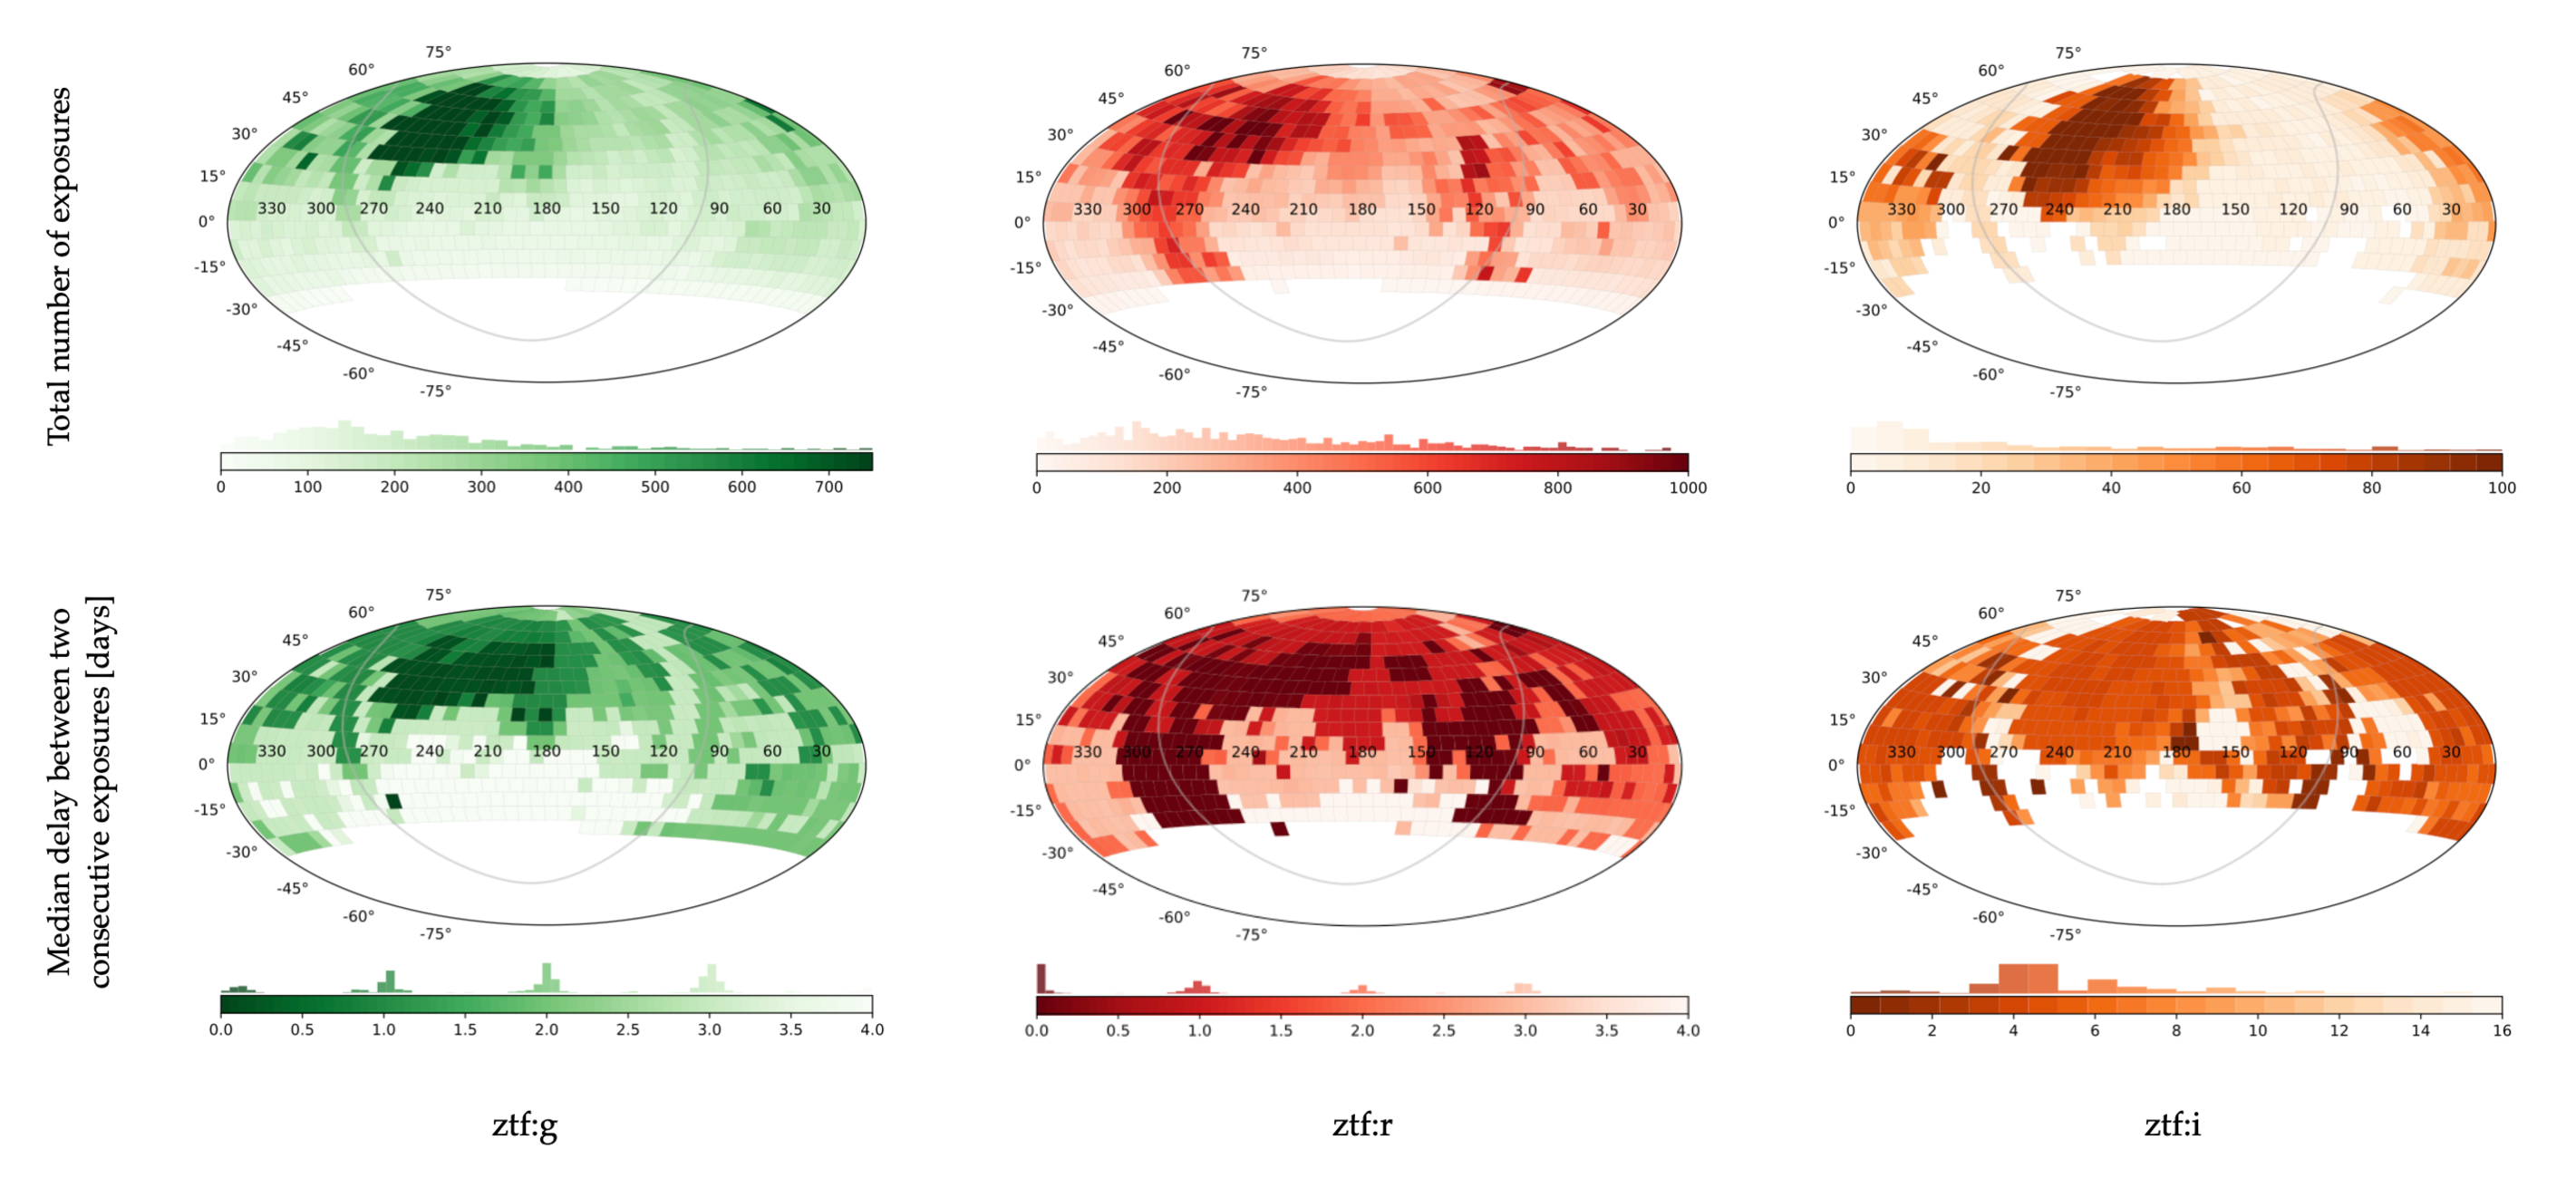
\includegraphics[width=1.15\textwidth]{../figures/09_dr2/ztf_skycoverage_and_cadence_landscape_lowq.pdf}}%
  \caption[Statistiques de la couverture du ciel de la phase 1 de
  ZTF.]{Statistiques de la couverture du ciel de la phase 1 de ZTF, pour
    chaque bande et chaque champ. Seules les images remplisssant les
    seuils de qualité ($431,202$) sont considérées. La bande grise sur
    chaque image représente la Voie Lactée ($b=0$). \emph{En haut} nous
    montrons le nombre total d'exposition par champ et par
    filtre. \emph{En bas} est présenté le délai médian entre deux
    expositions successives. Figure de M.Rigault.}
  \label{fig:skycoverage}
\end{figure}

\section{Statistiques sur les supernovae de type Ia}
%\label{sec:xxx}

\subsection{Classification spectrale}
%\label{ssec:xxx}

Seules les SNeIa ayant été classifiées spectralement sont considérées
dans la DR2. Nous montrons dans la Figure~\ref{fig:specorigindr2} la
distribution de tous les spectres appartenant à la DR2, répartis par
l'instrument de classification, et la quantité de SNeIa individuelles.
La DR2 complète, sans restriction de qualité sur les courbes de
lumières, est composé de $3742$ supernovae de type Ia, pour lesquelles
$5763$ spectres ont été extraits et utilisés pour la classification.
Environ $61.7\%$ des spectres ont été obtenus avec la SEDm, et donc
extraits par \hypergal, ainsi qu'une proportion similaire ($61.5\%$) de SNIa
unique. 

Le reste des spectres proviennent d'autres relevés possédant un
spectrographe de plus haute résolution que la SEDm, et utilisés
occasionnellement par
l'équipe du groupe \textit{Bright Transient Survey} (BTS) ou via des
requêtes de membres de la collaboration ZTF. D'autres spectres sont
également rendus publique par certains programmes, comme par exemple
ePESSTO utilisant le \textit{New Technology Telescope} (NTT) \citep{Smartt2015}.

\begin{figure}[ht]
  \centering
  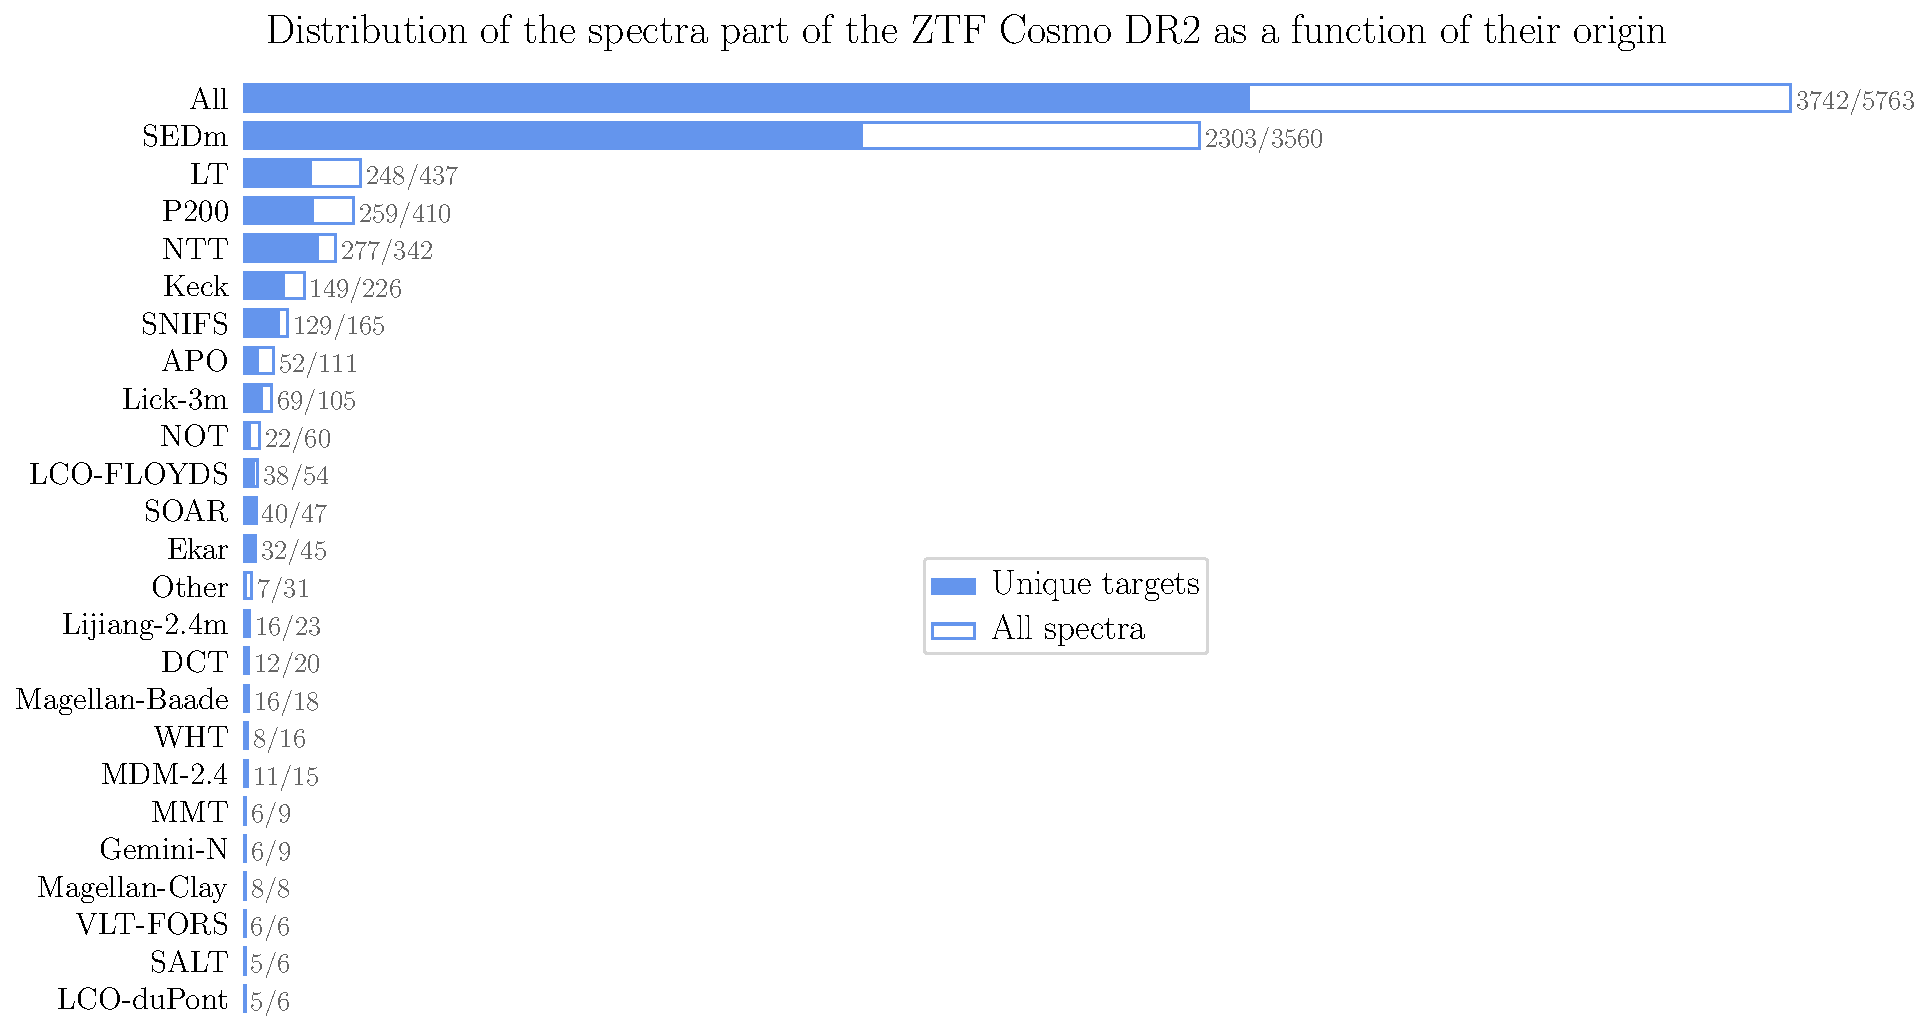
\includegraphics[width=1\textwidth]{../figures/09_dr2/spec_instorigin_dr2.pdf}
  \caption[Distribution des spectres appartenant à la DR2 de ZTF suivant
  leur origine.]{Distribution des spectres appartenant à la DR2 de ZTF suivant
  leur origine. Les barres entières de la figure indique la quantité de
  spectres extrait par tel ou tel instrument, la partie en bleue pleine
  indique le nombre de SNeIa unique correspondant. Une large majorité
  de spectre et de SNeIa ($\sim62\%$) ont été obtenues avec le spectrographe dédié à
  ZTF, la SEDm, et extraites par \hypergal. }
  \label{fig:specorigindr2}
\end{figure}

Près de $80\%$ de ces SNeIa font partie de l'échantillon BTS. Leur relevé
est conçu pour fournir un échantillon de supernovae purement limité par
leur magnitude ($m<19$ mag pour la détection, et $m<18.5$ mag pour la
classification), comme expliqué dans
\citet{FremlingZTFspec2020,PerleyBTSII2020}. Les SNeIa étant visibles
plusieurs semaines, la haute cadence des filtres $g$ et $r$ dans tout le
ciel Nord permet de n'en manquer que très rarement (caméra hors service,
ou mauvais temps sur une longue période par
exemple). \citet{PerleyBTSII2020} ont montré en se basant sur 25.5 mois
d'acquisition (ZTF MSIP de mars 2018 à mi-2020), que l'échantillon BTS
était spectroscopiquement complet à $97\%$, $93\%$ et $75\%$ aux
magnitudes limites $<18$ mag, $<18.5$ mag et $<19$ mag respectivement.

Dans notre cas, notre échantillon DR2 contient près de $20\%$ de SNeIa
supplémentaires à celui de BTS.

Nous montrons dans la Figure~\ref{fig:target_peakmaggBTS} le pic en
magnitude dans la bande $g$ de ZTF, dérivée à partir de l'ajustement
SALT2 des courbes de lumières sur les SNeIa (classifiées spectralement) de
la DR2. Nous montrons également la part de SNeIa appartenant également à
l'échantillon BTS par intervalle de magnitude. La fraction de SNeIa de
notre échantillon appartenant également à celui de BTS décroît fortement
aux magnitudes $>18.75$ mag, avant que les SNeIa uniques à la DR2
dominent clairement au delà de $19$ mag. Cette observation nous laisse
penser que notre échantillon de SNeIa est, à minima, spectroscopiquement
aussi complet que celui de BTS, et peut potentiellement être complet à $\sim100\%$
jusqu'à $18.75$ mag. On observe ensuite une décroissance brutale de cette complétude dans l'intervalle $18.75$-$19$ mag.

\begin{figure}[ht]
  \centering
  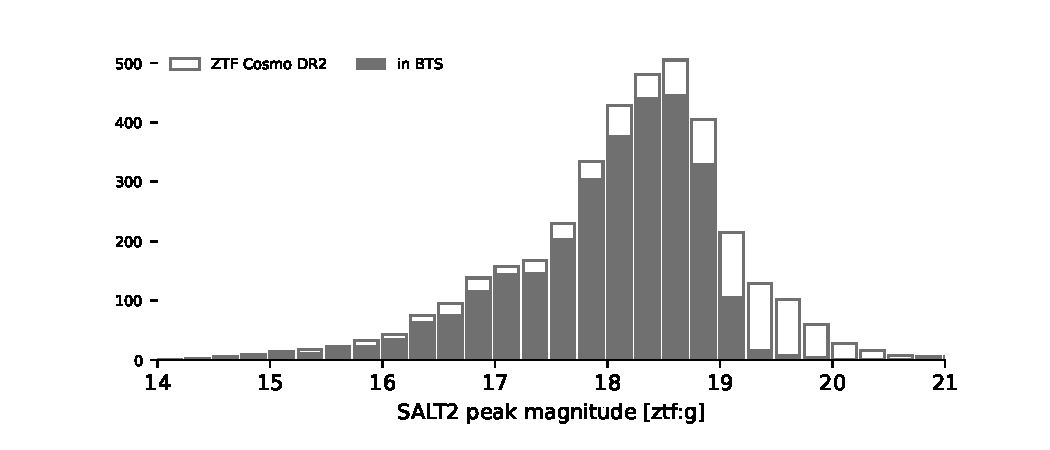
\includegraphics[width=1\textwidth]{../figures/09_dr2/target_peakmagg.pdf}
  \caption[Distribution du pic en
magnitude dans la bande $g$ de ZTF des SNeIa de la DR2.]{Distribution du pic en
magnitude dans la bande $g$ de ZTF des SNeIa de la DR2, dérivées à partir de l'ajustement
SALT2 des courbes de lumières. La partie noire de la distribution
correspond à la proportion de supernovae également incluses dans
l'échantillon BTS \citep{FremlingZTFspec2020,PerleyBTSII2020}. Figure de M.Rigault.}
  \label{fig:target_peakmaggBTS}
\end{figure}


\subsection{\textit{Golden sample}}

Nous allons nous concentrer dans la suite de ce chapitre sur le \textit{golden
  sample} de la DR2 de ZTF, sous-échantillon de la DR2 complète qui sera
utilisé pour la cosmologie. Cet échantillon est contraint par les
critères de qualité sur l'ajustement des courbes de lumière par SALT2
que nous avons détaillés au chapitre~\ref{ch:ztf} (détections
photométrique à $5\sigma$, $7$ points avant et $7$ points après le
maximum dans au moins $2$ bandes).
D'autres critères numériques sur la qualité d'ajustement des courbes de
lumière sont également
utilisés, que nous n'aborderons pas ici.

Nous montrons dans la Figure~\ref{fig:specorigingoldendr2} la nouvelle
distribution des spectres appartenant au \textit{golden sample} de la
DR2. Cet échantillon est composé de $2547$ supernovae de type Ia, pour lesquelles
$3903$ spectres ont été extraits et utilisés pour la classification.
Environ $65.1\%$ des spectres ont été obtenus avec la SEDm, et donc
extraits par \hypergal, ainsi qu'une proportion similaire ($65.3\%$) de SNIa
unique. 

\begin{figure}[ht]
  \centering
  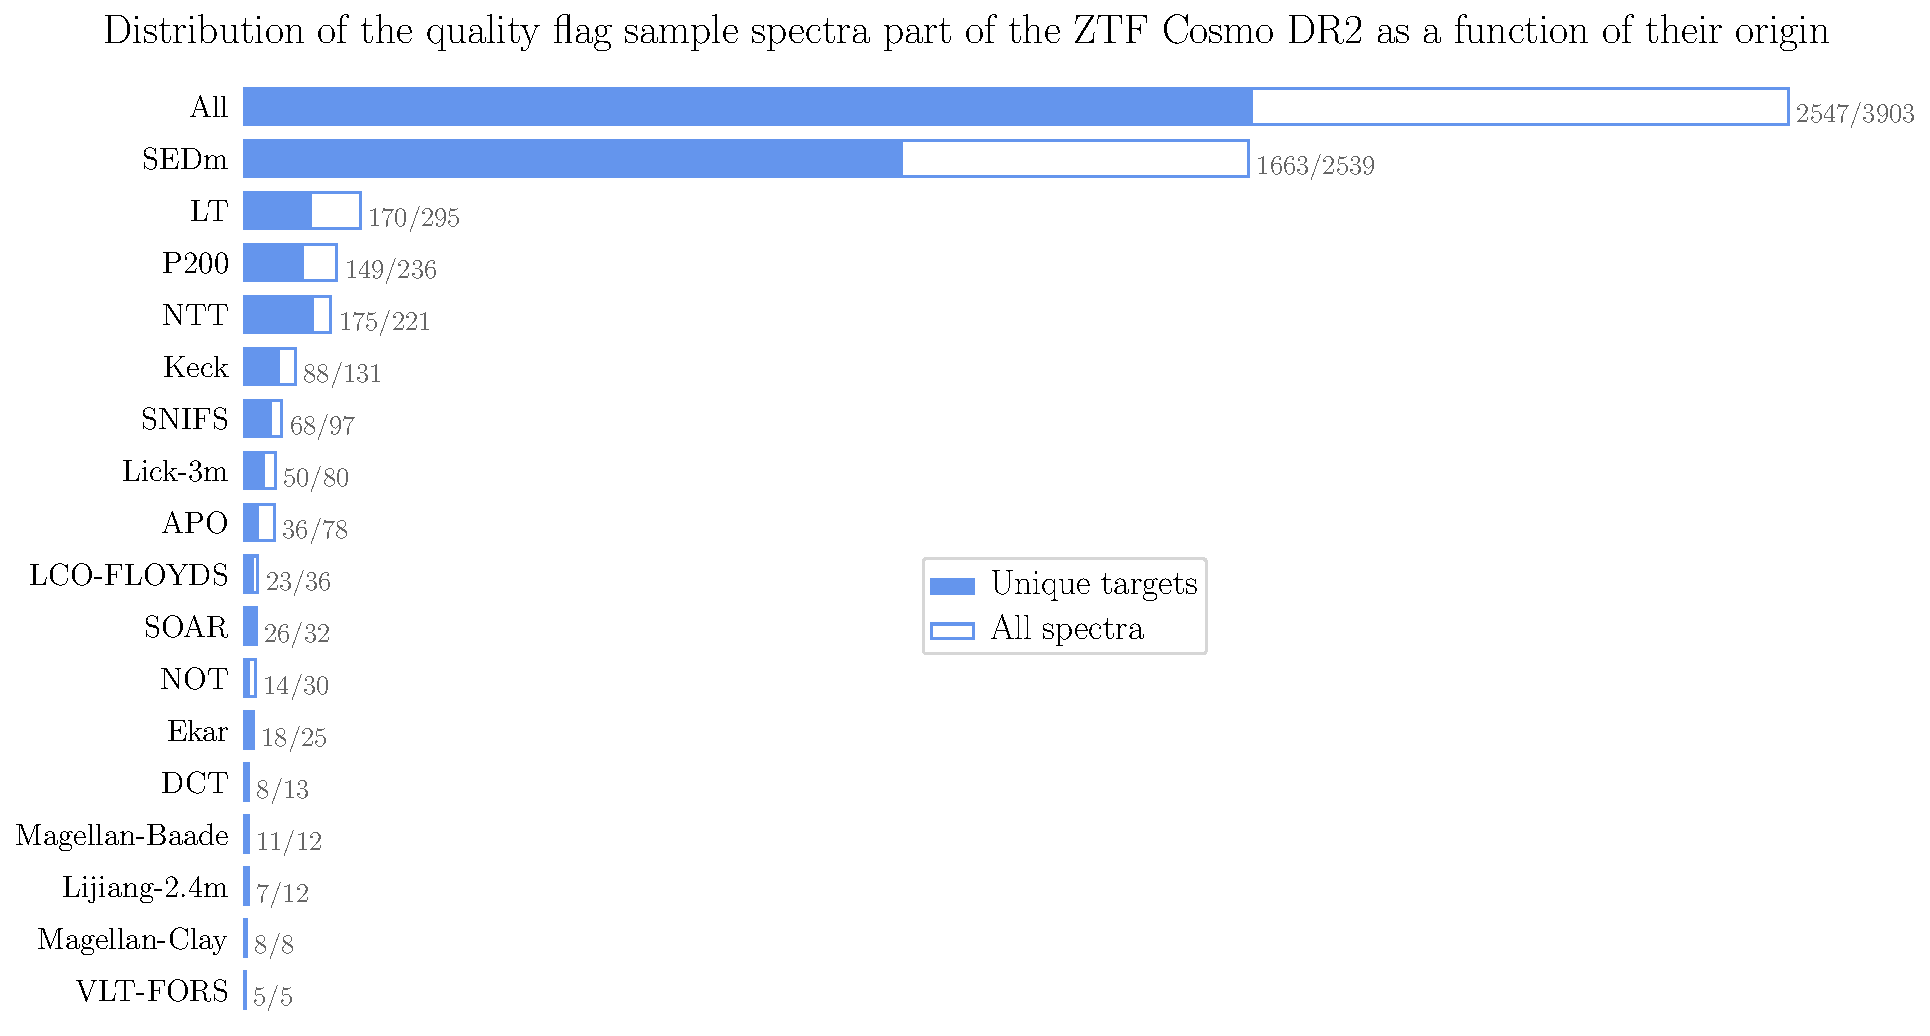
\includegraphics[width=0.9\textwidth]{../figures/09_dr2/spec_instorigin_golden_dr2.pdf}
  \caption[Distribution des spectres appartenant au \textit{golden sample} de la DR2 de ZTF suivant
  leur origine]{Distribution des spectres appartenant au \textit{golden
      sample} de la DR2 de ZTF
    suivant 
    leur origine. Les barres entières de la figure indique la quantité de
    spectres extrait par tel ou tel instrument, la partie en bleue pleine
    indique le nombre de SNeIa unique correspondant. Une large majorité
    de spectre et de SNeIa ($\sim65\%$) ont été obtenues avec le spectrographe dédié à
    ZTF, la SEDm, et extraites par \hypergal.}
  \label{fig:specorigingoldendr2}
\end{figure}


Nous montrons dans la Figure~\ref{fig:rlapdistribution} la distribution
en r$lap$ du meilleur modèle de SNID ayant permis la classification des
spectres du \textit{golden sample} de la DR2 de ZTF. La distribution de ce paramètre de qualité obtenue avec
\hypergal\ est similaire à celle obtenue avec les spectres extraits par d'autres
instruments, avec une moyenne (médiane) de r$lap\approx16(15)$, bien
supérieur au seuil de qualité de $5$.

\begin{figure}[ht]
  \centering
  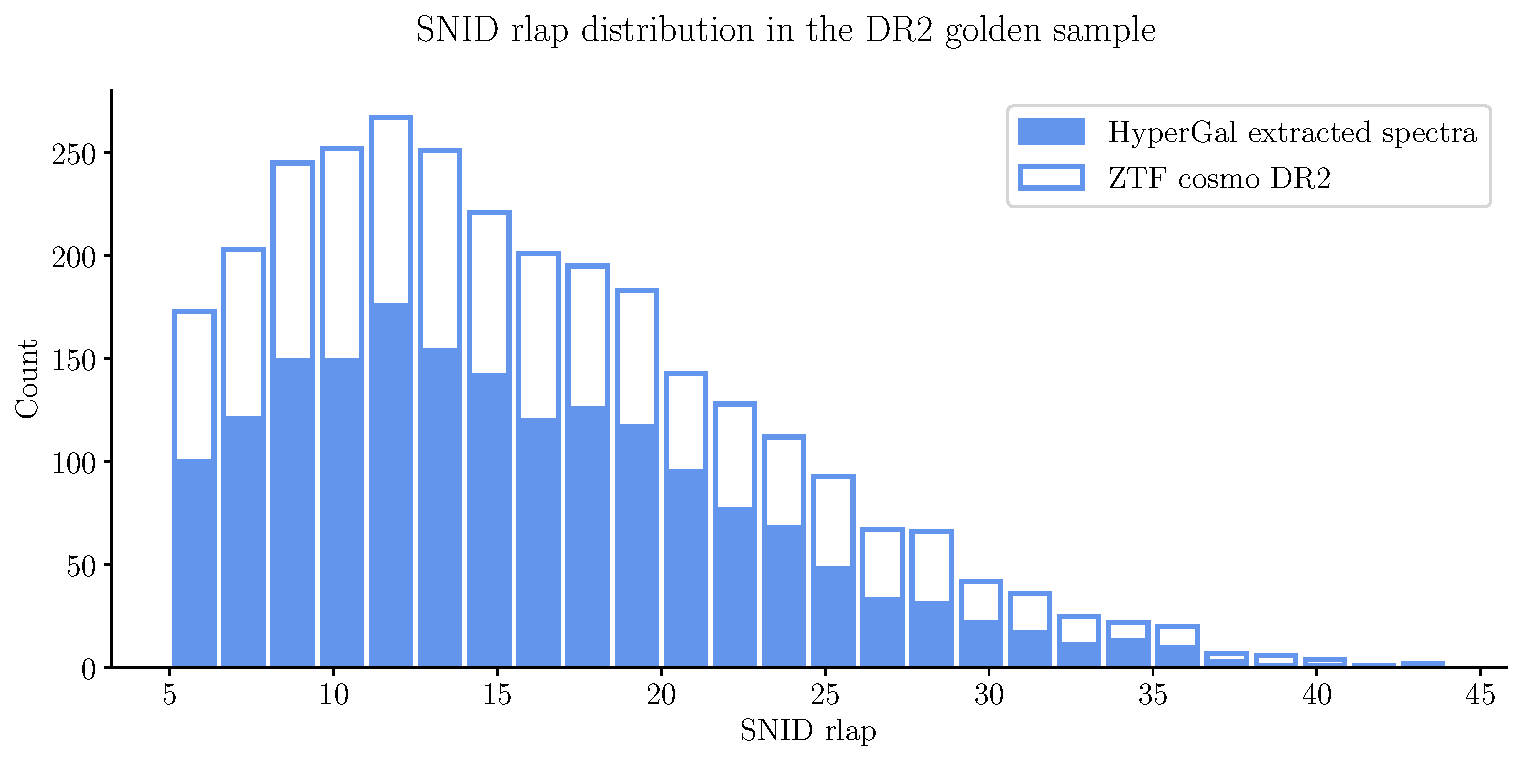
\includegraphics[width=0.75\textwidth]{../figures/09_dr2/rlapdistribution_dr2.pdf}
  \caption[Distribution du paramètre r$lap$ des meilleurs modèles
  \pkg{SNID} pour les spectres du \textit{golden sample} de la DR2 de ZTF.]{Distribution du paramètre r$lap$ des meilleurs modèles
  \pkg{SNID} pour les spectres du \textit{golden sample} de la DR2 de
  ZTF. En bleu sont présentés les spectres extraits par \hypergal\ et
  l'histogramme complet contient l'échantillon entier. }
  \label{fig:rlapdistribution}
\end{figure}


Cette quantité de spectre recueilli dans un même échantillon est sans
précédent, et va potentiellement permettre de mieux comprendre la
physique des supernovae de type Ia. Nous montrons dans la
Figure~\ref{fig:specexamplehypergal} un jeu de spectres de
différentes SNeIa extraits avec \hypergal, au maximum de luminosité (phase $=0$ jours) et
dans un même intervalle de redshift ($0.05<z<0.06$). 

\begin{figure}[ht]
  \centering
  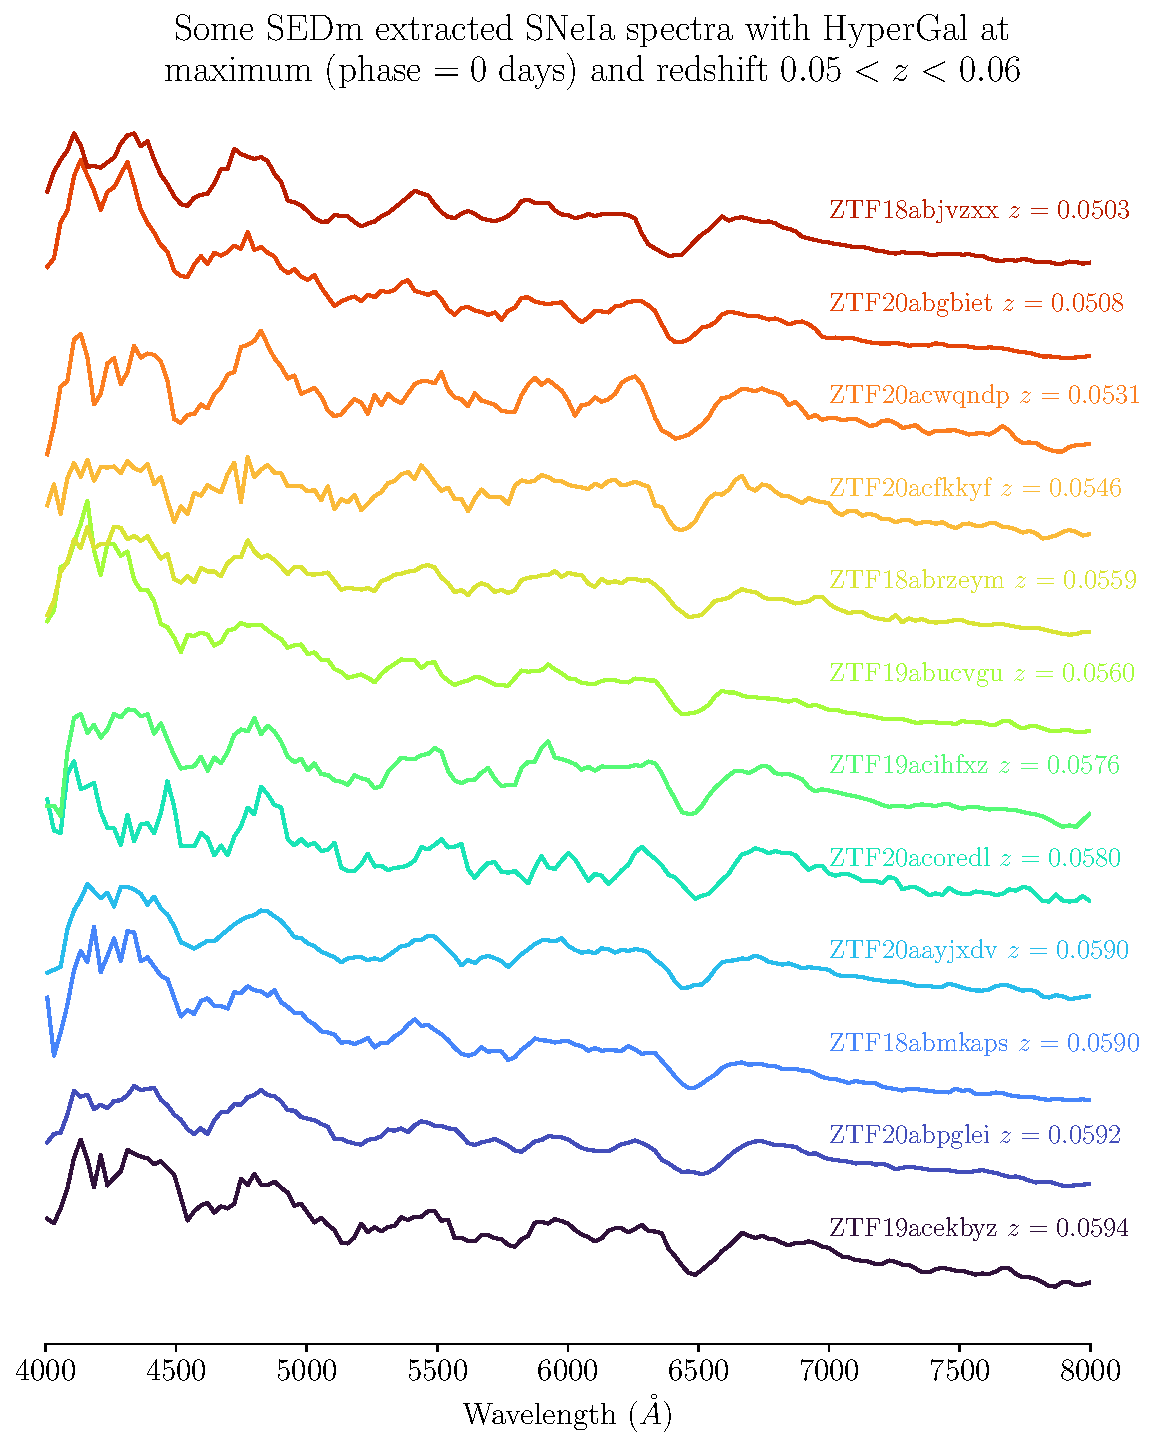
\includegraphics[width=0.7\textwidth]{../figures/09_dr2/spec_example_hypergaldr2.pdf}
  \caption[Exemple de spectres du \textit{golden sample} de la DR2
  extraits par \hypergal.]{Exemple de spectres du \textit{golden sample} de la DR2
  extraits par \hypergal\ au pic de luminosité dans un même intervalle
  de redshift ($0.05<z<0.06$).}
  \label{fig:specexamplehypergal}
\end{figure}



\subsection{Redshift et profondeur}
% \label{ssec:xxx}


Comme expliqué au chapitre~\ref{ch:ztf} présentant ZTF, seules
$\sim40\%$ des SNeIa possèdent un redshift spectroscopique provenant de
leur galaxie hôte (principalement du relevé spectroscopique SDSS). Les
redshift manquant proviennent des caractéristiques spectrales des SNeIa
à hauteur de $\sim50\%$, ou de raies d'émission de contamination de la
galaxie hôte ($\sim10\%$). Cependant, les redshifts obtenus par le
spectre des SNe sont précis à environ $5$\textperthousand, suffisant pour
certaines études (hôte-corrélation, populations ...) mais insuffisant
pour la cosmologie. Cependant, plus de $95\%$ des galaxies hôtes ont une
magnitude supérieur à $20$ mag, ce qui signifie que d'autres relevés (comme par
exemple DESI) pourraient à posteriori mesurer et fournir les redshift
manquant.

Nous montrons dans la Figure~\ref{fig:peakmagztfg} la corrélation
redshift/pic de magnitude (ZTF$_{g}$) ainsi que leur distribution pour
le \textit{golden sample} de la DR2.
Afin de mettre en évidence le rôle de la SEDm, nous indiquons en bleu toutes les SNeIa dont le spectre a été extrait par
\hypergal\ et en rouge toutes celles extraites avec un autre instrument.

La distribution des magnitudes au maximum n'est pas sans rappeler celle
de l'échantillon complet, présenté précédemment dans la Figure~\ref{fig:target_peakmaggBTS}.
À la profondeur limite de $19$ mag, les SNeIa observées avec la SEDm et
classifiées par \hypergal\
sont clairement dominantes, à hauteur de $\sim82\%$ ($1778/2182$). Nous
voyons d'ailleurs clairement sur la figure
la coupure à cette luminosité. Au delà de $19$ mag, nous observons une dominance nette des
SNeIa classifiées par d'autres instruments, la SEDm ne contribuant alors que
pour seulement $31\%$ de SNeIa au delà de cette magnitude. De façon
générale, la quantité de SNeIa dans l'échantillon
tout instrument confondu croît 
continuellement jusqu'à $18.5$ mag, pour
ralentir à $18.75$ mag et décroitre brusquement de $50\%$ au delà de $19$
mag.

La distribution en redshift croît continuellement jusqu'à $z<0.07$,
avant de décroître progressivement. En suivant la méthode présenté par
\citet{NoraNicolas21} pour obtenir un échantillon de SNeIa dans un
volume limité mais complet, nous trouvons que l'échantillon cosmologique
DR2 de ZTF devrait être libre de fonction de sélection jusqu'à un
redshift de $z=0.06$. La fonction de sélection sera activement discuté dans
l'article de \mbox{\textsc{Amenouche} et al. (in prep.)}.

Ce volume limité est composé de $949$ SNeIa, dont $181$ provenant d'une
classification hors SEDm, et $768$ provenant d'une
classification SEDm+\hypergal, soit $\sim81\%$ de ce sous échantillon.

\begin{figure}[ht!]
  \centering
  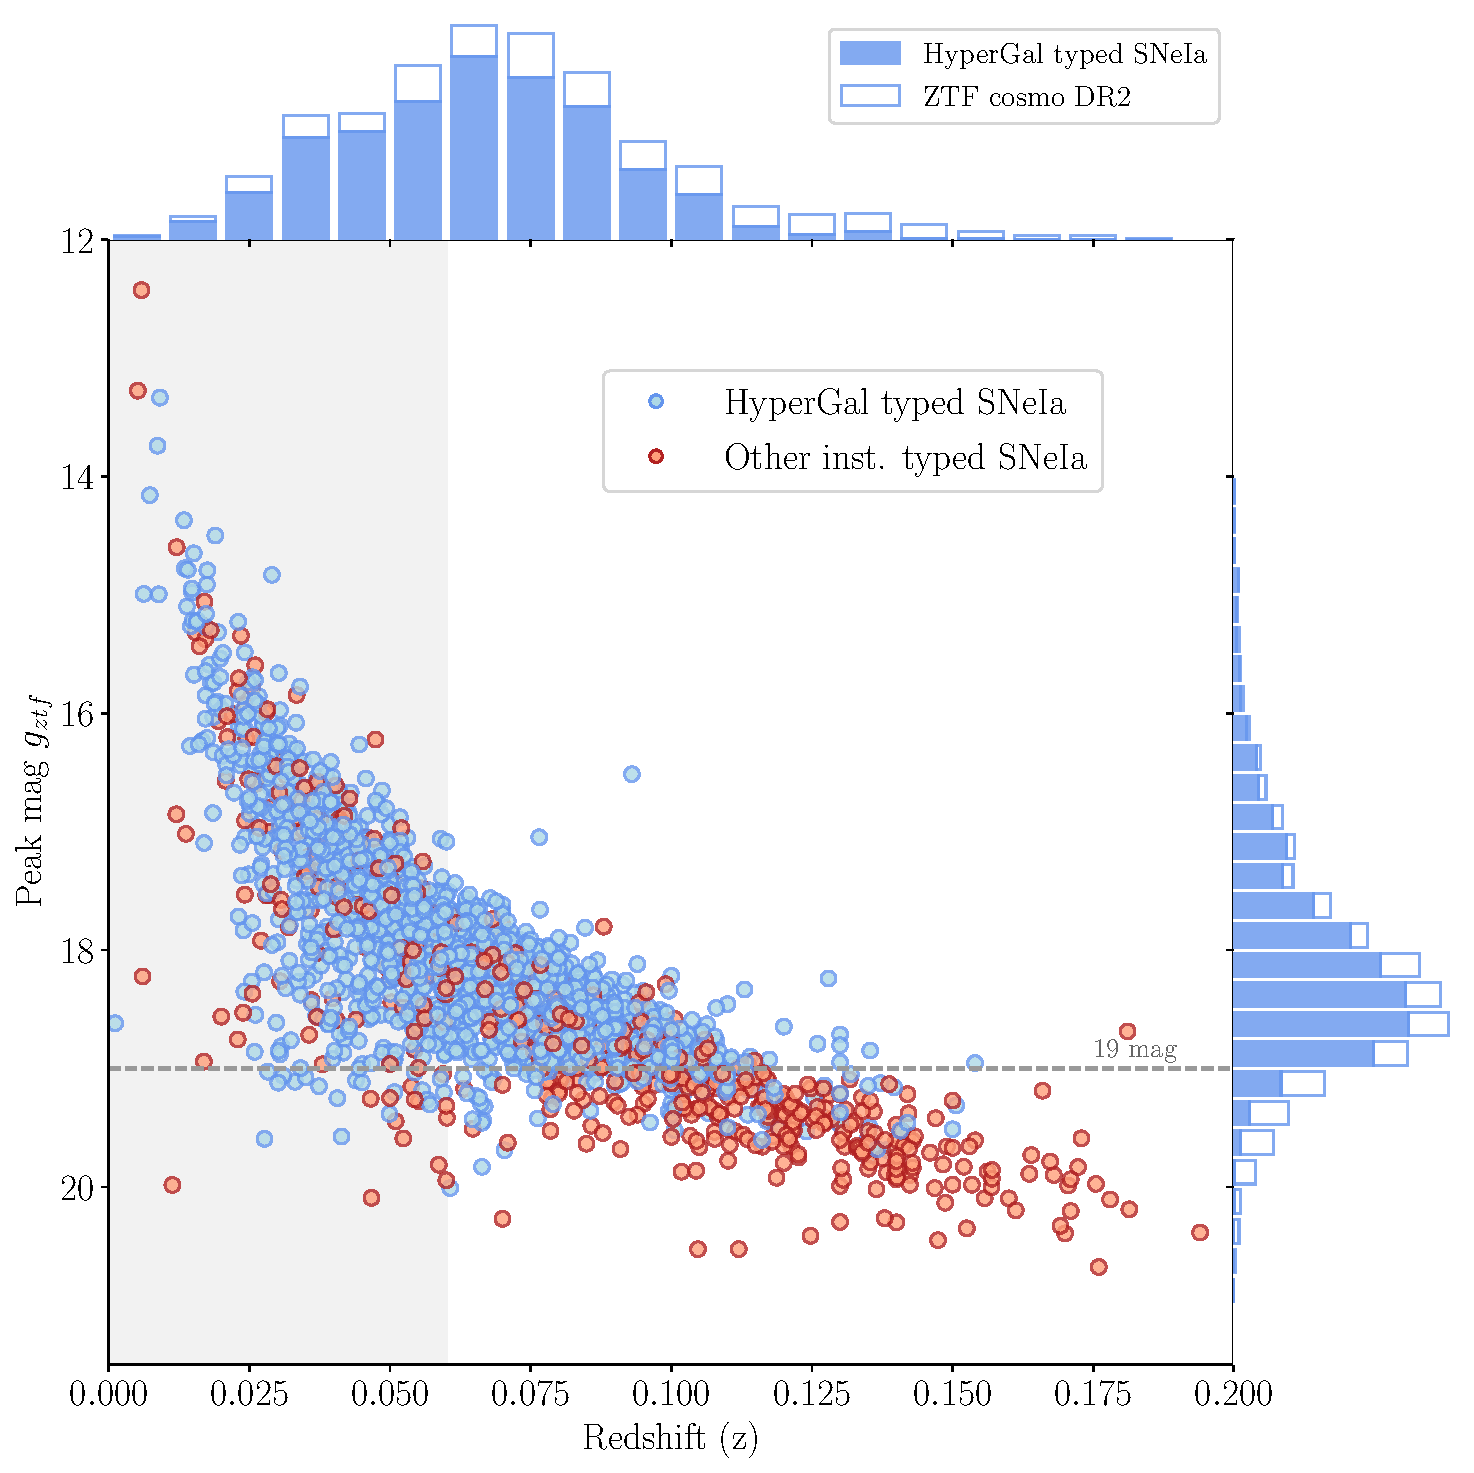
\includegraphics[width=1\textwidth]{../figures/09_dr2/peakvsredshift_dr2.pdf}
  \caption[Corrélation redshift/pic de magnitude (ZTF$_{g}$) du
  \textit{golden sample} de la DR2 de ZTF.]{Corrélation redshift/pic de
    magnitude dans la bande ZTF$_{g}$ des SNeIa du
  \textit{golden sample} de la DR2 de ZTF. Nous indiquons la limite à
  $19$ mag, limite à laquelle la vaste majorité des classifications a
  été effectuée grâce à la SEDm, et a fortiori \hypergal. La bande grise
 indique le sous échantillon à volume limité au redshift $z=0.06$,
 profondeur où l'échantillon est potentiellement libre de fonction de sélection.}
  \label{fig:peakmagztfg}
\end{figure}

\clearpage
\subsection{Courbes de lumière}

\subsubsection{Phases}
Nous présentons ici quelques résultats préliminaires obtenus à partir de
l'ajustement des courbes de lumière avec SALT2, en restant
focalisé sur le \textit{golden sample} de la DR2. La
Figure~\ref{fig:lc_example} illustre à titre d'exemple la courbe de lumière de trois
SNeIa, avec l'ajustement SALT2 correspondant. La première correspond à
une SNIa observée à très haute cadence, avec plus d'une centaine de
points avant et après le maximum de luminosité. La seconde présente un
cas typique des SNeIa de la DR2, avec un dizaine de points avant le pic,
et une quinzaine après. Le troisième exemple illustre un cas limite du
seuil de qualité pour appartenir au \textit{golden sample} de la DR2.

\begin{figure}[ht!]
  \centering
  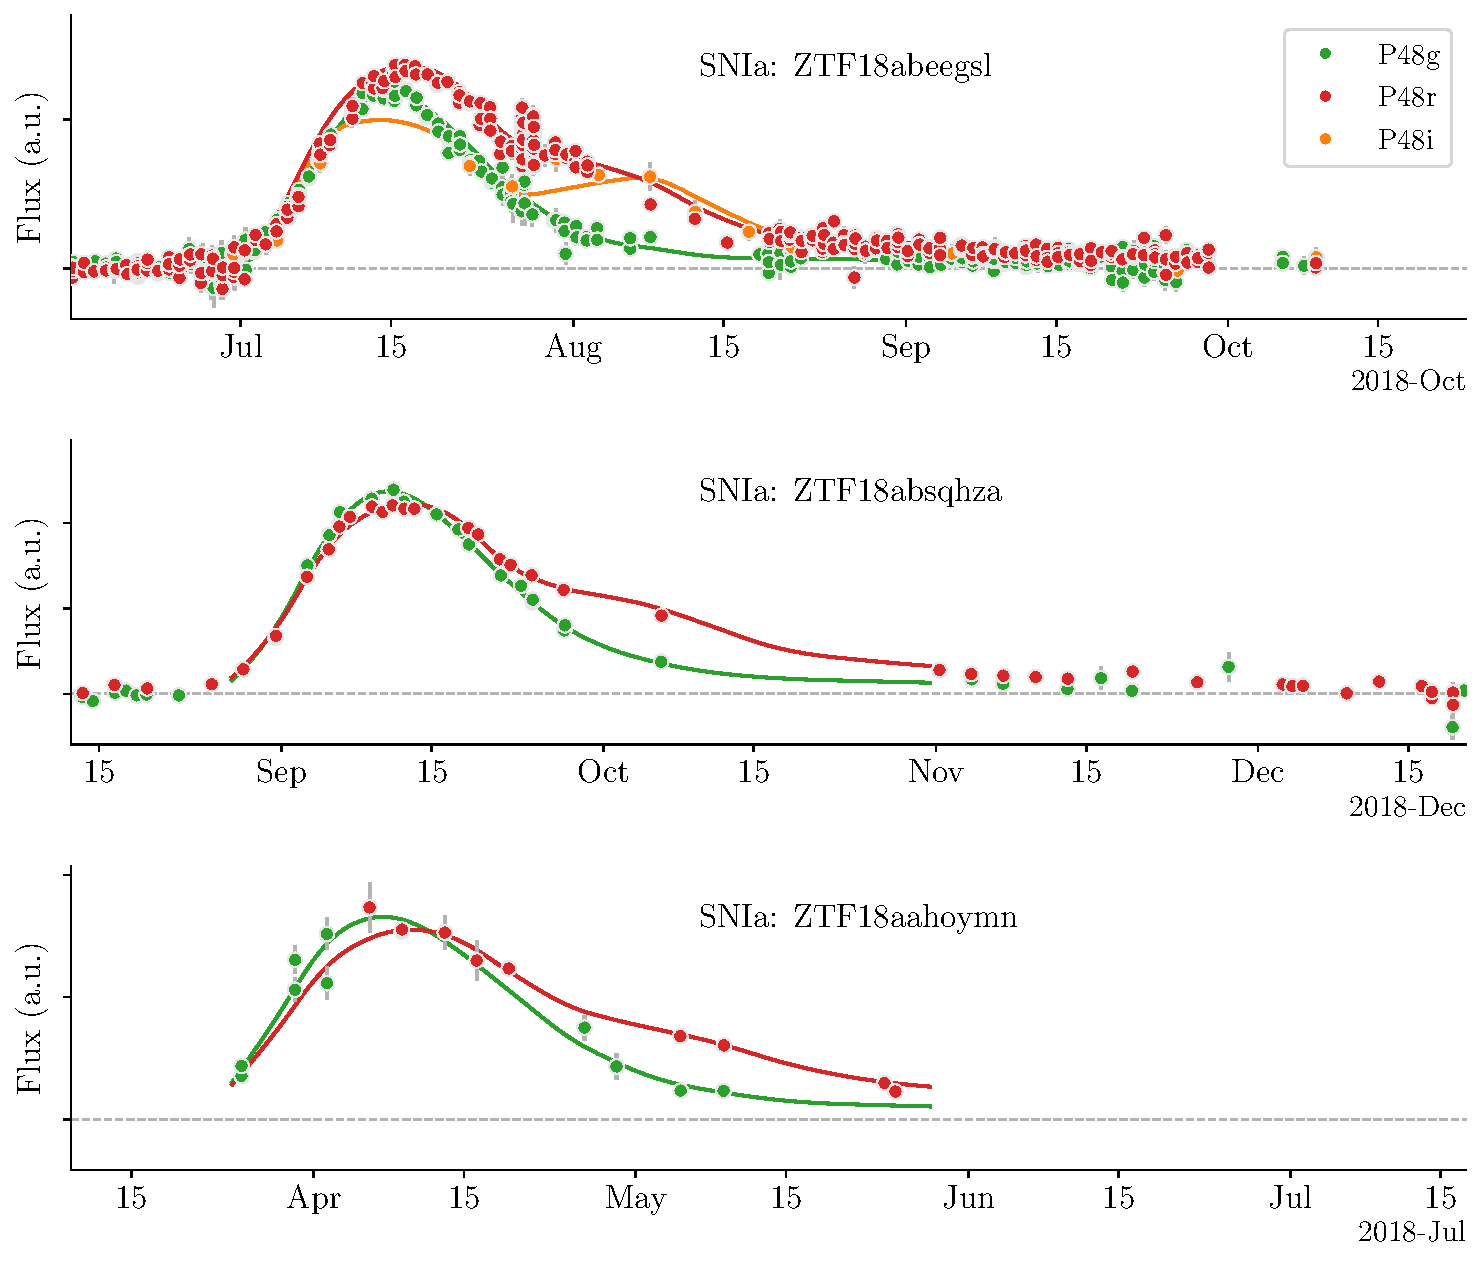
\includegraphics[width=0.97\textwidth]{../figures/09_dr2/lightcurve_example_dr2.pdf}
  \caption[Exemple de courbe de lumière de SNeIa du \textit{golden
    sample} de la DR2.]{Exemple de courbe de lumière de SNeIa du
    \textit{golden sample} de la DR2. Nous montrons également
    l'ajustement SALT2 correspondant. Le code couleur réfère à la bande
    de ZTF considérée. De \emph{haut en bas}: Un cas extrême de très
    haute cadence avec plusieurs centaines de points, un cas typique
    avec une dizaine (quinzaine) de points avant (après) le maximum, et
    un cas limite pour intégrer notre échantillon.}
  \label{fig:lc_example}
\end{figure}

La distribution du nombre de points de détection avant et après le
maximum est présentée dans la Figure~\ref{fig:earlylatephase}, où nous
restreignons la partie \textit{early phase} à une phase comprise entre
[-20d, 0d], et la partie \textit{late phase} entre [0d, +30d]. Nous
voyons bien que, typiquement, nous avons $\sim10$ points avant le
maximum de luminosité, et $\sim20$ points après. La première détection
photométrique survient à une phase médiane de $-13.3$ jours toutes bandes
confondues ($-12.3$ pour $g$, $-12.5$ pour $r$ et $-8$ pour $i$).
\begin{figure}[ht!]
  \centering
  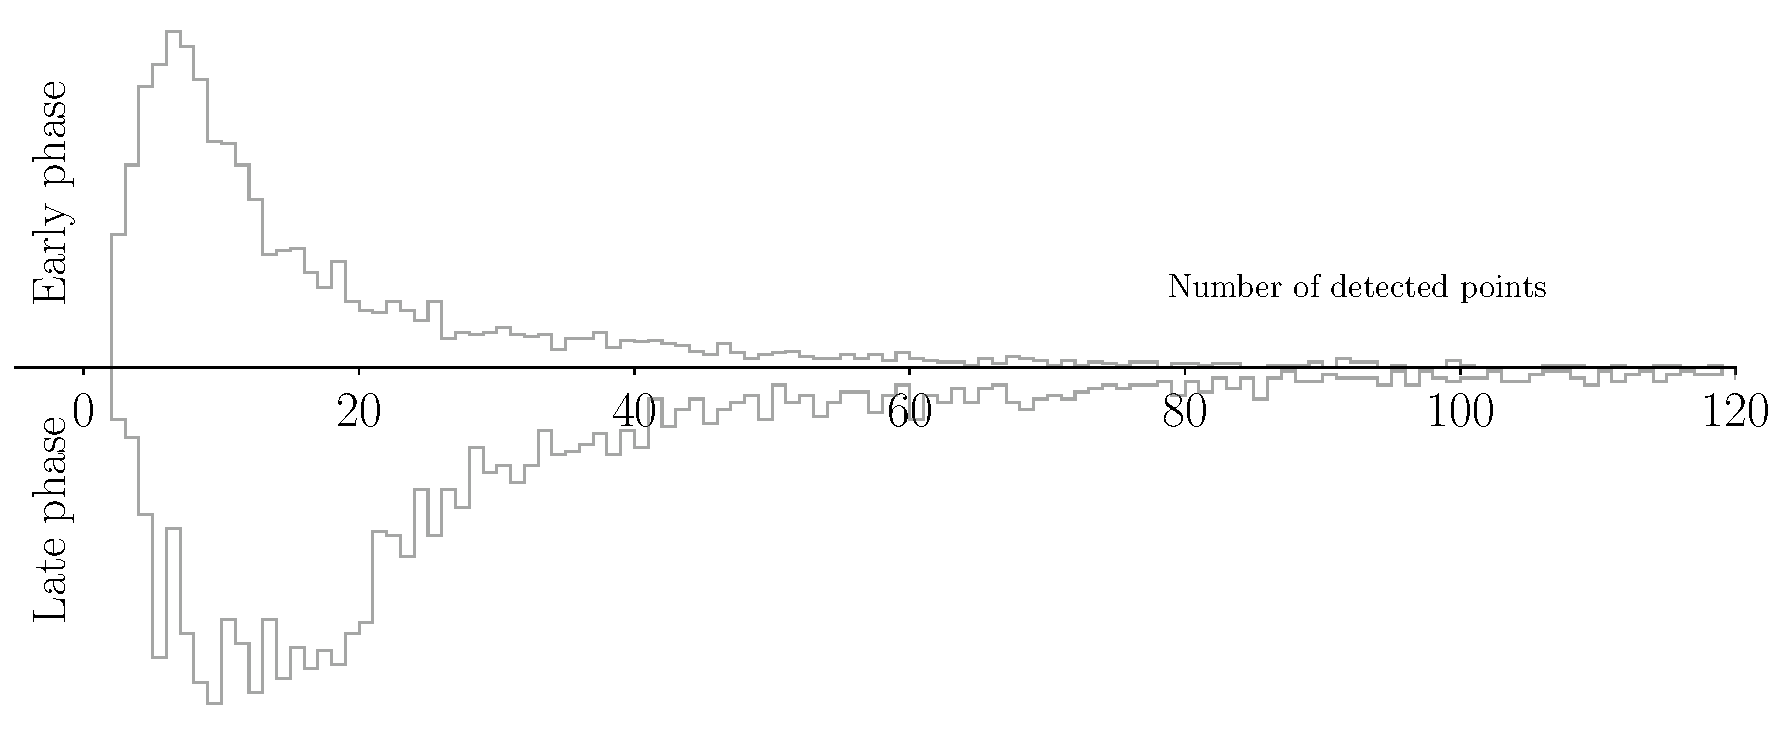
\includegraphics[width=0.9\textwidth]{../figures/09_dr2/early_late_phase_dr2.pdf}
  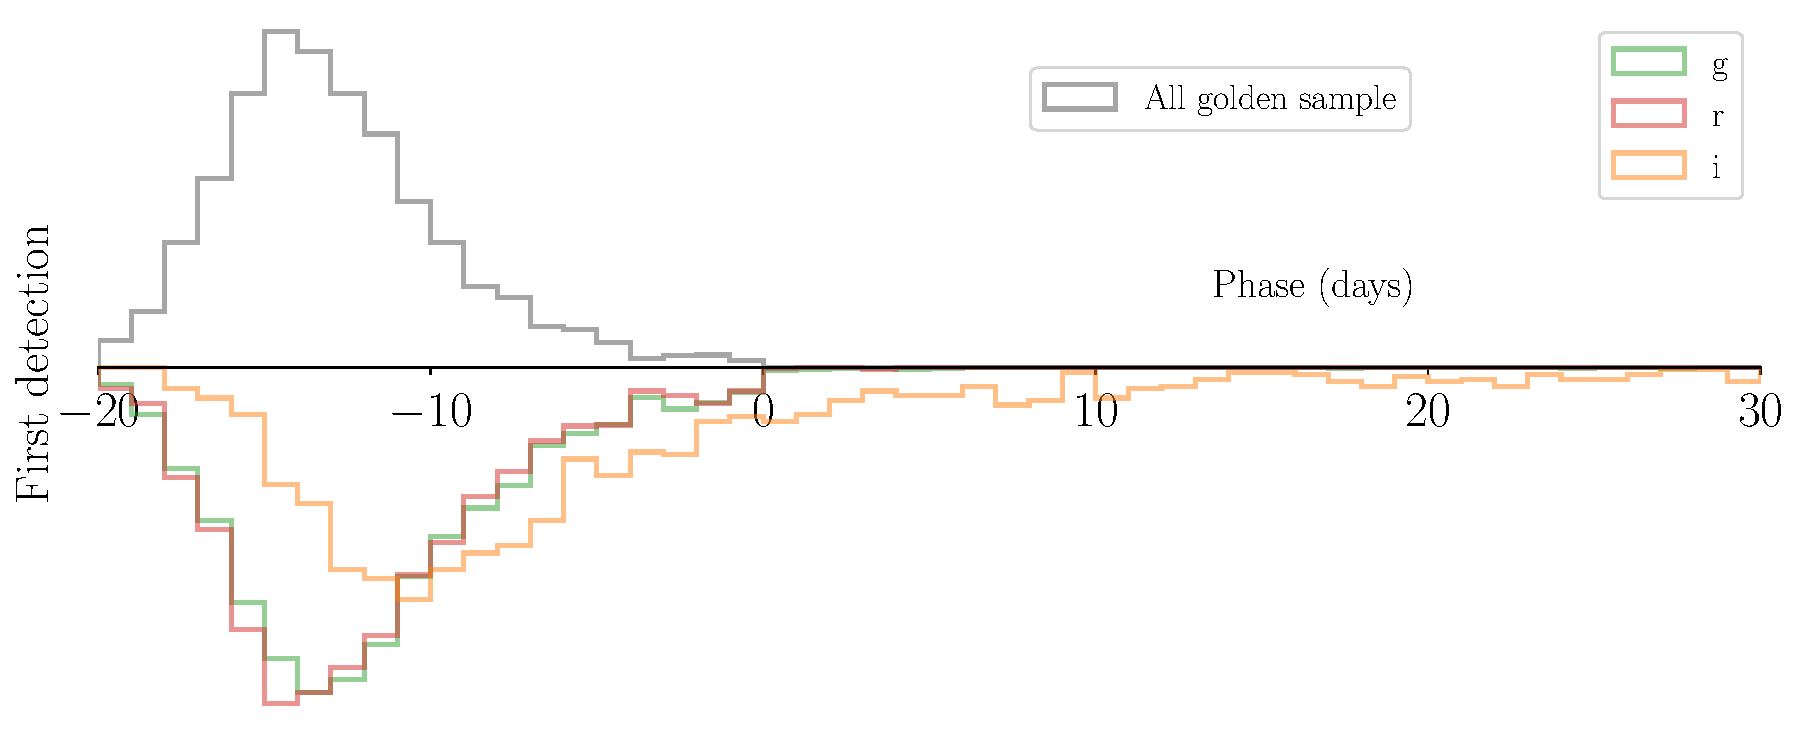
\includegraphics[width=0.9\textwidth]{../figures/09_dr2/first_detect_dr2.pdf}
  \caption[Distribution de points de détection avant/après le maximum de
  luminosité et distribution de phase de la première détection du
  \textit{golden sample} de la DR2.]{\emph{En haut}: distribution du
    nombre de
    points de détection photométrique (toutes bandes confondues) avant et après le maximum de
  luminosité pour les SNeIa du
  \textit{golden sample} de la DR2. Nous avons typiquement $\sim10$ points avant le
maximum de luminosité, et $\sim20$ points après. \emph{En bas}:
distribution de phase de la première détection photométrique pour le
même échantillon, toutes bandes confondues (en gris) et dans chaque
bande individuelle (couleurs). La première détection survient à une phase médiane de $-13.3$ jours.}
  \label{fig:earlylatephase}
\end{figure}


Nous montrons également la distribution de phase lors de la première
acquisition spectrale dans la Figure~\ref{fig:phaseIa}, en distingant la
SEDm des autres instruments. La SEDm est l'instrument
le plus réactif pour obtenir le premier spectre des SNeIa de notre
échantillon, avec $\sim70\%$ de premières détections. Les spectres
de première détection ont une phase médiane de $-3$ jours, soit environ
$10$ jours après la première détection photométrique.

\begin{figure}[ht]
  \centering
  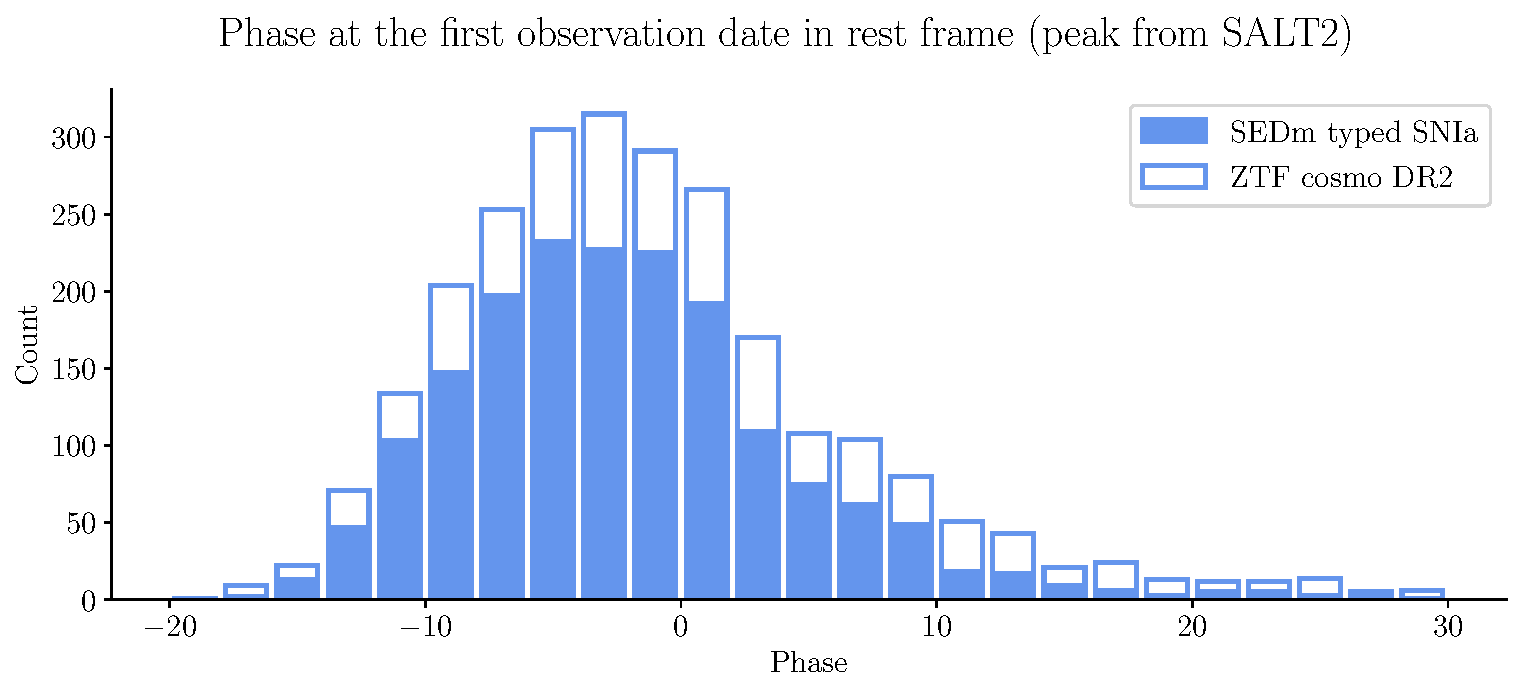
\includegraphics[width=0.9\textwidth]{../figures/09_dr2/phaseIadr2.pdf}
  \caption[Distribution de phase de la première acquisition spectrale
  des SNeIa de la DR2.]{Distribution de phase de la première acquisition spectrale
  des SNeIa de la DR2. La partie bleue pleine de la distribution indique
la proportion de spectre extraite par la SEDm, et a fortiori \hypergal,
comme toute première extraction spectrale.}
  \label{fig:phaseIa}
\end{figure}


Il est par ailleurs possible de comparer les phases obtenues avec SALT2
avec celles obtenues avec \pkg{SNID} sur les spectres de SNeIa, et donc
indépendamment des observations photométriques. Nous montrons cette
relation dans la Figure~\ref{fig:snid_vs_salt_phase}. Pour cette étude,
nous avons considéré tous les spectres du \textit{golden sample}, en
distanguant ceux acquis avec la SEDm des autres instruments. Pour la
phase, nous avons utilisé celle du meilleur modèle ajusté par
\pkg{SNID}. Nous observons que la qualité des spectres, tout instrument
confondu, permet de retrouver une phase à environ $\pm3$ jours de celle
obtenue avec SALT2, avec moins d'une dizaine de valeurs aberrantes
parmi les milliers de spectres analysés.

\begin{figure}[ht]
  \centering
  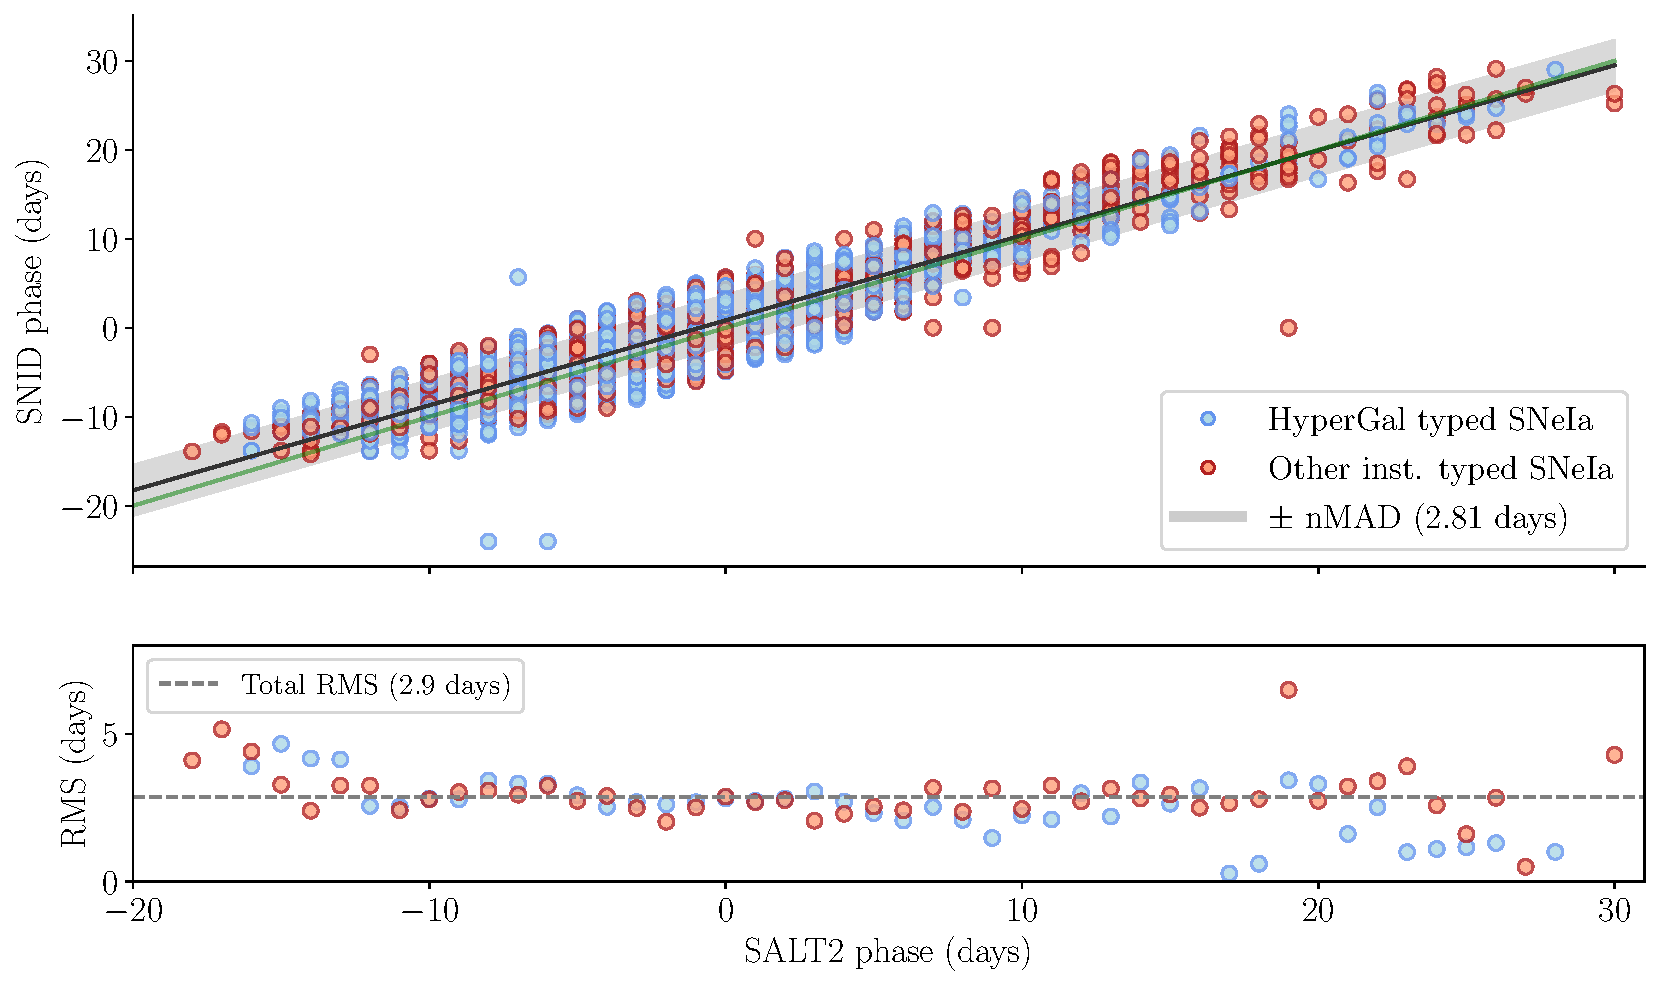
\includegraphics[width=0.9\textwidth]{../figures/09_dr2/snidphase_vsphase_dr2.pdf}
  \caption[Corrélation phases SNID vs phases SALT2 de la DR2 de
  ZTF.]{\emph{En haut}: corrélation entre les phases SNID et les phases SALT2 du
    \textit{golden sample} de la DR2 de ZTF. Nous indiquons avec la
    ligne verte la fonction identité, et en noir l'ajustement linéaire
    et le nMAD comme estimateur de la déviation standard. En bas nous
    montrons le RMS par intervalle ($1$ jour) de phase déterminé avec
    SALT2, sachant la date d'acquisition spectrale. Les spectres
    semblent permettre de déterminer la phase avec une précision de
    l'ordre de $\pm3$ jours.}
  \label{fig:snid_vs_salt_phase}
\end{figure}


%\clearpage
\subsubsection{\textit{Stretch} ($x_{1}$) et couleur ($c$)}

L'ajustement des courbes de luminosité avec SALT2 nous permet de
remonter aux paramètres de standardisation, le \textit{stretch} $x_{1}$
et la couleur $c$, intrinsèques à chaque SNIa.

Nous commençons par illustrer dans la Figure~\ref{fig:ztfdr2salt} la
corrélation de chacun de ces deux paramètres avec le redshift, en
considérant le \textit{golden sample} dans son ensemble. La corrélation
en redshift est clairement visible dans les deux cas, et nous observons
clairement un nombre décroissant de SNeIa observées à bas
\textit{stretch} (déclin rapide de luminosité), et de couleur élevée
(plus rouges). La bande grise indique à nouveau la profondeur en
redshift du volume limité ($z<0.06$), et l'observation de ces
corrélations nous conforte sur cette hypothèse d'échantillon libre de
fonction de sélection à cette profondeur.

Nous faisons également la distinction dans cette figure des SNeIa
observées par la SEDm (extraites par \hypergal) et celles extraites par
d'autres instruments. Nous voyons nettement la dominance de la SEDm pour
la classification des spectres
jusqu'à un redshift d'environ $z\approx0.1$ ($80\%$; $1760/2205$ SNeIa),
du même ordre de grandeur que dans
l'échantillon à volume limité ($81\%$). Au delà de $z=0.1$, la majorité
des SNeIa ($65\%$) ont été classifiées à partir d'un spectre obtenu d'un autre
instrument, possédant une plus haute résolution et surtout une plus
grande profondeur.

\begin{figure}[ht]
  \centering
  \makebox[\textwidth][c]{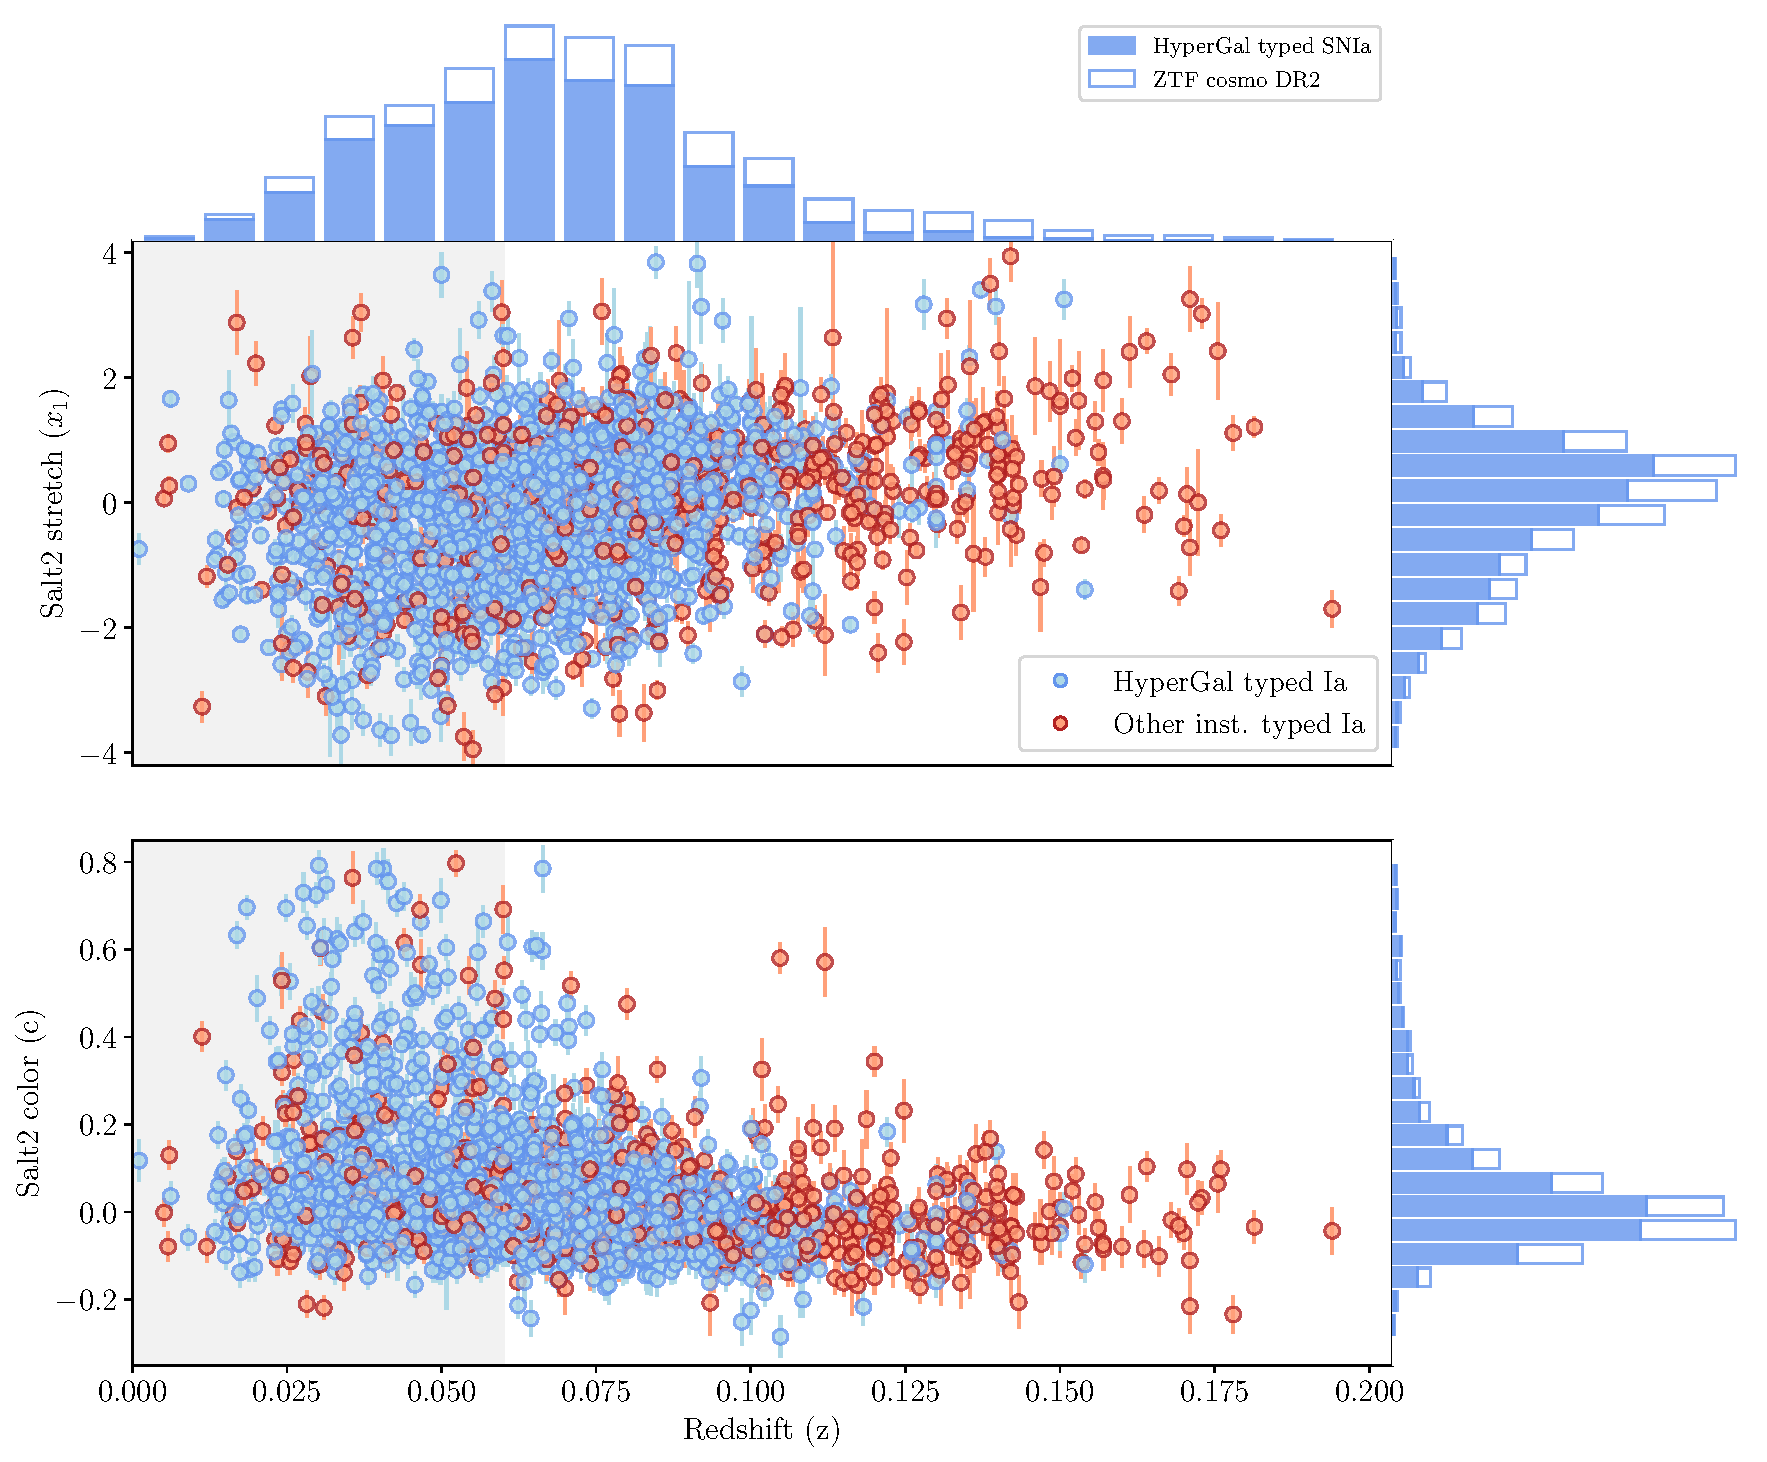
\includegraphics[width=1.1\textwidth]{../figures/09_dr2/stretch_color_redshift_dr2.pdf}}%
  \caption[Paramètres SALT2 de stretch et couleur pour la DR2 de
  ZTF]{Paramètres SALT2 de stretch $x_{1}$ (\emph{en bas}) et couleur $c$
    (\emph{en haut}) pour la DR2 de ZTF. Seules les SNeIa du
    \textit{golden sample}
    sont considérées. La bande grise indique le
    volume limité à $z<0.06$. Les points bleus (histogrammes bleus)
    correspondent aux SNeIa ayant été classifiées suite à une extraction
    spectrale avec la SEDm. Les points rouges (histogrammes blancs)
    correspondent aux SNeIa classifiées par un autre instrument. Nous
    voyons clairement l'autosuffisance de la SEDm jusqu'à un redshift
    $z\approx0.1$, au delà duquel la majorité des SNeIa ont été
    classifiées par un autre spectrographe.}
  \label{fig:ztfdr2salt}
\end{figure}

En se focalisant à présent sur l'échantillon à volume limité, nous
pouvons alors plus clairement étudier la distribution des paramètres des courbes de
lumière $x_{1}$ et $c$, sans se soucier\footnote{Cette hypothèse est bien évidemment encore à
valider par \mbox{\textsc{Amenouche} et al. (in prep.)}} d'effets de sélection pouvant
affecter la dérivation des paramètres cosmologiques
\citep{Scolnicbias2016}.

En supposant que ce sous-échantillon est effectivement libre de fonction
de sélection, alors l'étude des paramètres des courbes de lumière nous
offrirait deux informations importantes. Premièrement, la distribution
de ces paramètres nous permettrait
de faire une estimation précise de la fonction de sélection à utiliser
pour l'échantillon entier. Dans un second temps, cette étude nous donne les
clés pour étudier la nature de la population de SNeIa, et sonder une potentielle
évolution avec le redshift \citep{NoraNicolas21}.



Nous présentons les corrélations \textit{stretch}/couleur de
l'échantillon à volume limité
dans la Figure~\ref{fig:ztfdr2saltcorr}. Comme précédemment, nous
distingons les SNeIa classifiées avec la SEDm des autres
instruments. Nous montrons ainsi les distributions en \textit{stretch}
et en couleur pour le sous-échantillon entier (en gris), et pour les SNeIa
classifiées par la SEDm seules (en bleu). Les distributions sont
présentés sous forme \textit{d'idéogrammes}, déterminés à partir de la
somme des contributions gaussiennes définies par chaque point de donnée
et l'erreur associée. Ces idéogrammes pemettent ainsi de représenter au
mieux la distribution des données en supposant une erreur gaussienne, et
de façon continue (sans intervalle contrairement à un histogramme
classique). Chaque idéogramme est normalisé de sorte que l'intégrale
soit unitaire. Nous pouvons ainsi clairement voir que la distribution
des paramètres des courbes de lumières appartenant aux SNeIa classifiées
par la SEDm sont parfaitement représentatifs de l'échantillon dans son ensemble. 

Par ailleurs, nous pouvons voir que la caractéristique bi-modale
de la distribution en stretch est clairement visible. Le mode à bas
\textit{stretch} compte pour $\approx25\%$ de la distribution, comme prédit par
\citet{NoraNicolas21}, dont nous présentons l'ajustement sur les données
en superposition à l'idéogramme.

\begin{figure}[ht]
  \centering
  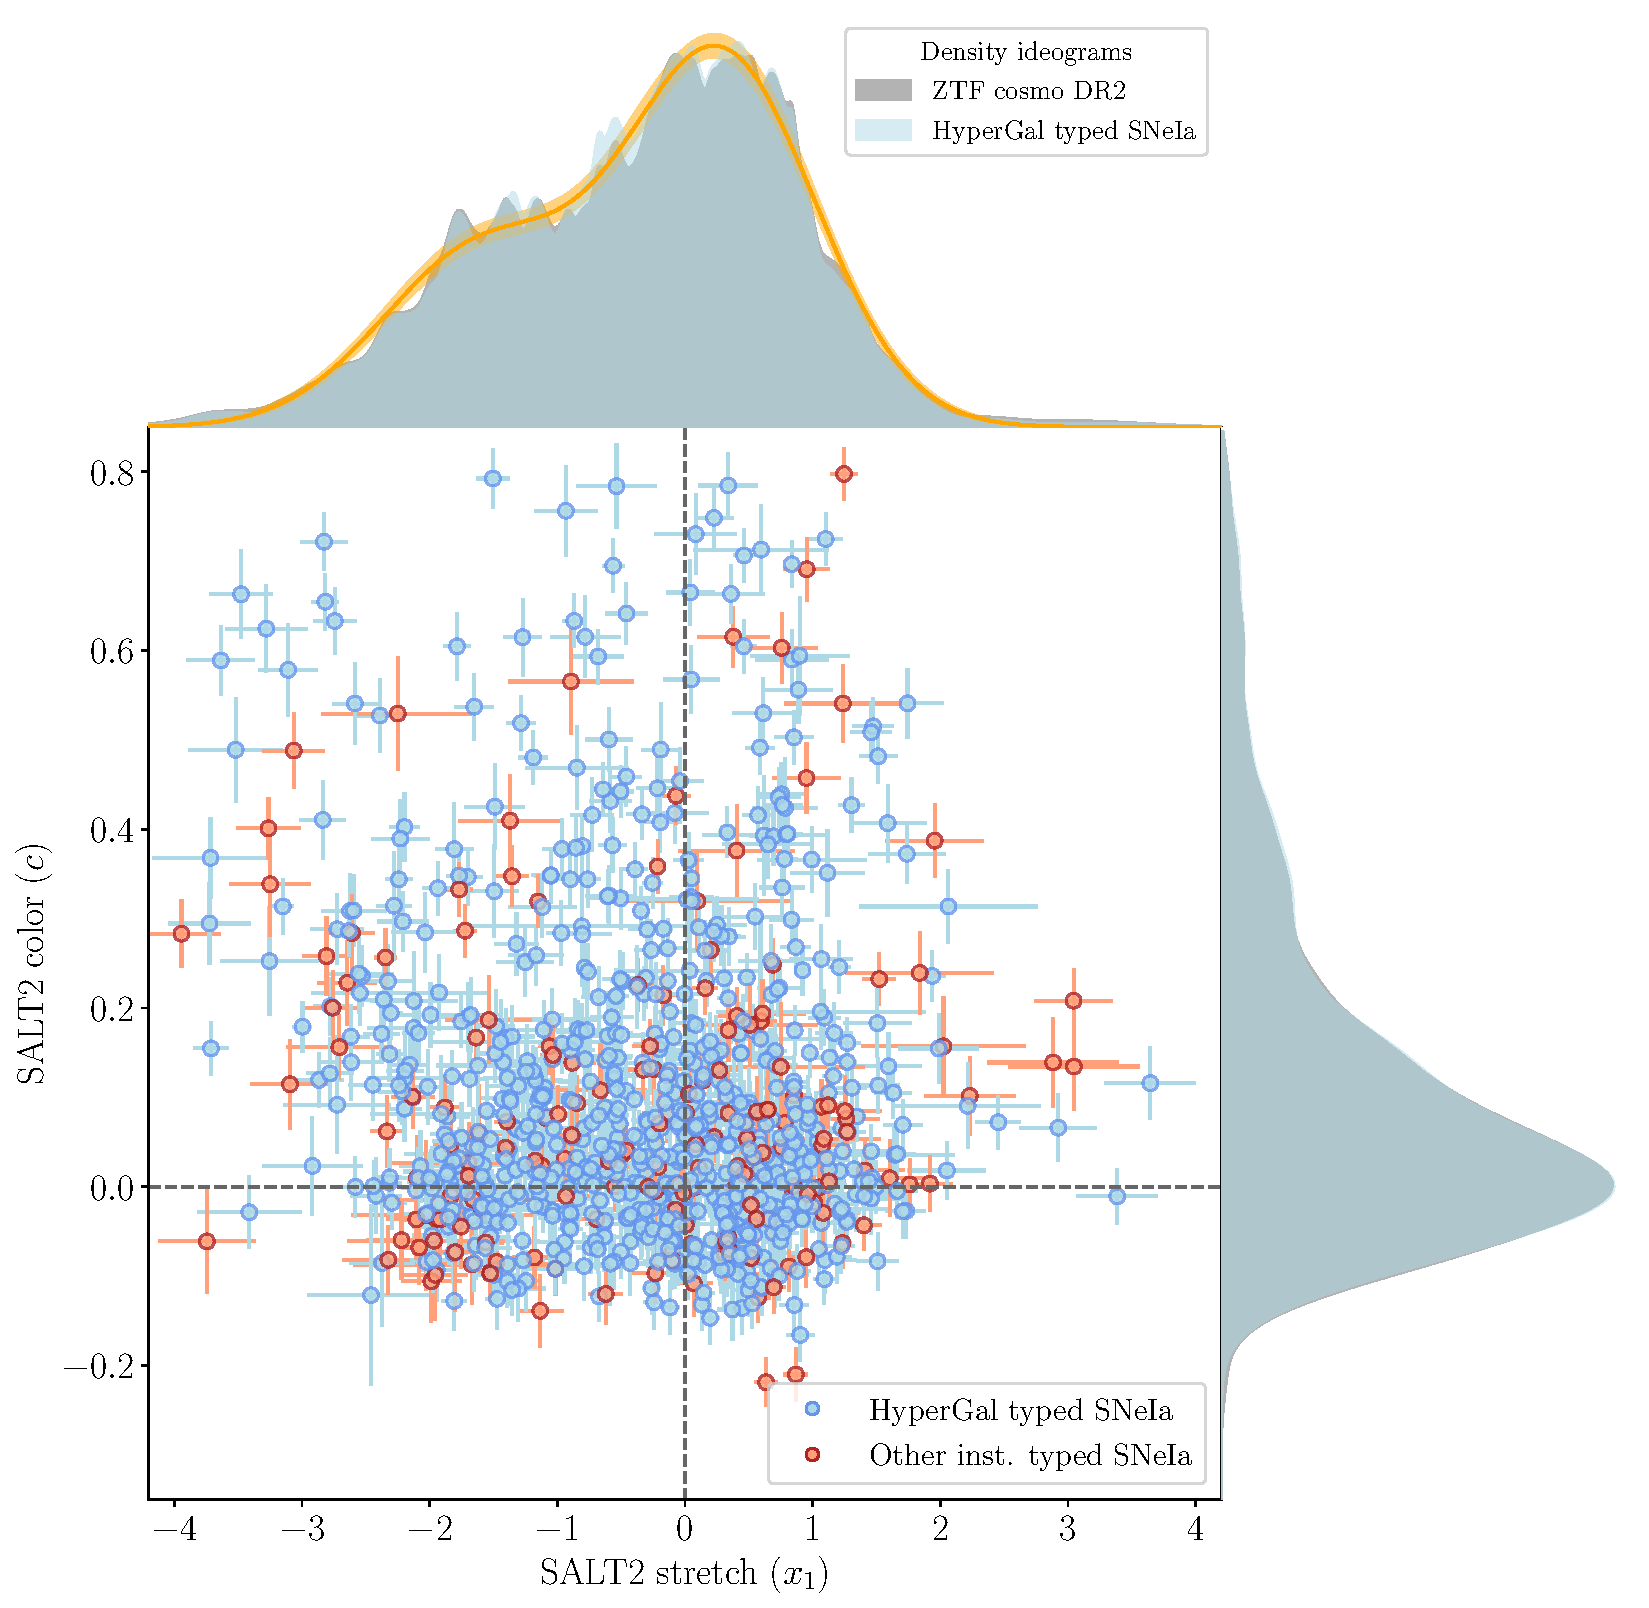
\includegraphics[width=1.1\textwidth]{../figures/09_dr2/stretch_color_driftmodel_dr2}
  \caption[Correlation entre les paramètres SALT2 de \textit{stretch} et
  couleur dans l'échantillon à volume limité.]{ Correlation entre les paramètres SALT2 de \textit{stretch} et
    couleur pour le \textit{golden sample} de la DR2 de ZTF. Ici seules les SNeIa du
    volume limité à $z<0.06$ sont considérées. Les points bleus 
    correspondent aux SNeIa ayant été classifiées suite à une extraction
    spectrale avec la SEDm. Les points rouges
    correspondent aux SNeIa classifiées par un autre instrument. Les
    distributions de chaque paramètres sont représentées sous forme
    d'idéogramme, déterminés à partir de la
    somme des contributions gaussiennes définies par chaque point de donnée
    et l'erreur associée. Chaque idéogramme est normalisé de sorte que l'intégrale
    soit unitaire. Les distributions bleues représentent la contribution de
    la SEDm, et les grises celles sans distinction d'instrument ayant
    classifié la SNIa. Nous voyons clairement l'illustration de
    l'auto-suffisance de la SEDm pour représenter la population de SNeIa
    dans ce volume limité. La courbe orange correspond au modèle bi-modal
    redshift dépendant de \citet{NoraNicolas21}.}
  \label{fig:ztfdr2saltcorr}
\end{figure}

\clearpage
\section{Conclusion}

La DR2 de ZTF est composée de près de $3700$ SNeIa, dont $\sim2600$
remplissent les critères de qualité cosmologique. La vaste majorité de
cet échantillon à bas redshift de nouvelle génération proviennent de la
SEDm, spectrographe 3D dédié à la classification des SNe. L'utilisation
d'\hypergal\ dans cette data release a ainsi contribué à la
classification de $65\%$ des SNeIa la composant.

En se concentrant sur la limite en redshift de $z<0.1$, profondeur à
laquelle la SEDm a été conçue, ce sont près de $80\%$ des SNeIa de l'échantillon
qui ont été classifiées par \hypergal\ ($1760/2205$). Cela témoigne clairement du rôle
cruciale de la SEDm dans l'utilisation de cette sonde cosmologique.

L'étude des paramètres des courbes de lumières et de la distribution en
redshift des SNeIa du \textit{golden sample} de la DR2 pointent vers
l'existence d'un sous-échantillon dans le volume limité $z<0.06$
complet, libre de toute fonction de sélection, et entièrement réalisé
avec le même instrument. Ce volume limité est constitué à $81\%$
($768/949$) de SNeIa observées par la SEDm et classifiées par
\hypergal.
D'ici la fin de la seconde phase de ZTF (ZTF-II; décembre 2020 -
mi-2024), il est attendu que le \textit{golden sample} passe de
$\approx2600$ SNeIa à plus de $5000$ SNeIa, toutes classifiées
spectralement et dans les même proportions qu'actuellement par \hypergal, et
remplissant les critères de qualité pour la dérivations de paramètres cosmologiques.

%\clearpage
%\section{Vers la cosmologie}\label{sec:sniaztfcosmo}

%\subsection{Taux d'expansion ($H_{0}$)} 

%\subsection{\'Equation d'état de l'énergie sombre ($w$)}

%\subsection{Taux d'accroissement des structures ($f\sigma_{8}$)}


%\bibliographystyle{../main/aa_url2}
%\bibliography{99_references}
\end{document}

%%% Local Variables:
%%% mode: latex
%%% TeX-master: t
%%% End:
